\chapter{Review of Cystic Fibrosis and The Molecular Basis of its Treatment}
\label{chap:cftr}
\chapquote{Because of what's inside me; Because of my genes.}{-Bob Flanagan \cite{dick1997}.}
\newpage
%Authors note:
% We begin with a breif overview of the disease Cystic Fibrosis as it is the main motiation for this project. A horrendous disease for which we will hopefully soon find a cure.

%Clinical outcomes are a chronic illness which affects multiple organ systems and every aspect of a patient's life. 
	%physical therapy, pancreatic sufficiency, ongoing discovery of chronic issues. Much to do. 


% The cause of the disease is CFTR misfunction.
       % CFTR function overview

% CFTR modulators act to restore its function. 
	% patients with rare genotypes cant access modulators.

This thesis primarily focusses on the molecular causes of Cystic Fibrosis (CF). In subsequent chapters we will use Molecular Dynamics (MD) to determine what kind of defect rare mutations cause to the Cystic Fibrosis Transmembrane conductance Regulator (CFTR), the gene whose mutation causes CF. We do this with the goal of understanding what kind of treatments rare disease causing mutations might respond to. Given the importance of the CFTR protein system to this work, we will look at its structure and dynamics in some detail in this chapter. In this chapter I have abandoned simple pedagogy in order to compile a detailed reference text for future endeavours into molecular studies of CFTR, perhaps even my own one day. To understand the motivation for this level of effort, we will first review some of the medical literature surrounding the disease itself. 

We will first look at some of the symptoms of living with the disease before we look at the structure and function of the CFTR protein---Noting how basic science discoveries and translational research have directly lead to better outcomes for patients. We will then once more work way upward, to understand the protein system and what causes it to misfunction, followed by the mechanism behind its restoration by small molecule drugs. We will show how to integrate this molecular perspective closely with \textit {ex vivo} organoid models which are grown from a patient's own cells. These organoid models be used in subsequent chapters to prove that small molecule drugs appear to be capable of treating a diverse set of molecular phenotypes. In chapter \ref{chap:conclusion} we will use these results to argue that this personalised approach to medicine leads us to expect that more patients with rare mutations will be able to benefit from modulator therapy. 

We will end the chapter with a brief overview of the different experimental techniques which were employed by collaborators of this thesis work to characterise the response of different mutations to different drugs. The language in these sections is kept simple, so the unfamiliar physicist reader can understand some of the common techniques they will encounter in the literature surrounding biochemistry and cell biology. The intention is not replication but comprehension, so a biochemist familiar with these procedures would likely find these explanations lacking. Where details are noted, it is with the intention for the reader to have access to a molecular detail in CFTR which has informed my thinking about the function the protein. Dry lab readers are encouraged to spend lots of time learning from their experimental colleagues or even perform some of these experiments themselves if possible. 

In previous chapters we always began with the smallest physically relevant length scale and then worked  upward. In chapter \ref{chap:methods} I showed how we can begin from Schr\"odinger's wave equation and work to build simulation techniques which let us understand whole biomolecular systems. This was to give an example of the philosophy I outlined in chapter \ref{chap:introduction}, where the physicist designs abstract formalisms and integrates them to model macroscopic physical phenomenon. By contrast, in this chapter we will begin with a discussion of the human reality of living with CF disease. We will then review its genetic cause and the molecular basis behind its treatment. I have taken particular care to begin this chapter with a discussion of the clinical outcomes of the disease we are studying, so we do not lose sight of our goals in biophysics research.

When one trains to practice medicine they are taught how to conduct themselves ethically, with their patients best interests at heart \cite{hajar2017}. Typically, a physicist has no such training and they may miss the human aspect of medicine by studying disease impersonally \cite{foucault1994}. 

We must be aware of the challenges that this represents. In the 20th century, physicists often participated in political and moral discourse, and not always for the better \cite{frank1993, gottfried1999, global2009, rhodes1986, aaronson2008, berger2016, vonneumann_britanica}. Should we wish to embark on the enterprise of studying biophysics we have a responsibility to also study how to do it ethically. Thankfully, many important questions have been studied by philosophers, so the reader is encouraged to seek texts on bioethics and also ethics in the use of artificial intelligence \cite{buchanan2000, taneri2011, genome_editting_guildelines_2017, muller2021, bostrom2014}. These considerations are likely to become increasingly important---as biophysics advances, so too does its capacity for misuse \cite{mallapaty2022, urbina2022}. 

%On this somewhat somber note, we will now take a brief look at what it is like to live with Cystic Fibrosis.

%We will then analyse the root cause, mutations to the Cystic Fibrosis transmembrane Conductance Regulator (CFTR). In chapter \ref{chap:conclusion} we will use much of the knowledge gained in this chapter to think about where we can direct future studies to help treat the root cause of Cystic Fibrosis. 

\section{Clinical Realities of Living with Cystic Fibrosis}
Cystic Fibrosis (CF) is the most common fatal genetic condition in Caucasian populations. Over 162 000 people are estimated to be afflicted globally, with a significant proportion living undiagnosed \cite{hammoudeh2021,guo2022}. Even with decades of research there is no known cure for CF patients and patients have a life expectancy below 50 \cite{mcbennett2022}. Management of disease symptoms also bears significant financial and emotional costs to patients and their families \cite{vangool2013, page2022}. From a cellular perspective, the symptoms of the disease are due to the inability of certain cells to regulate their salt content, causing an osmotic imbalance (Figure \ref{CF_summary}) \cite{reddy2013}. 

\begin{figure}
	\label{CF_summary}
	\begin{center}
	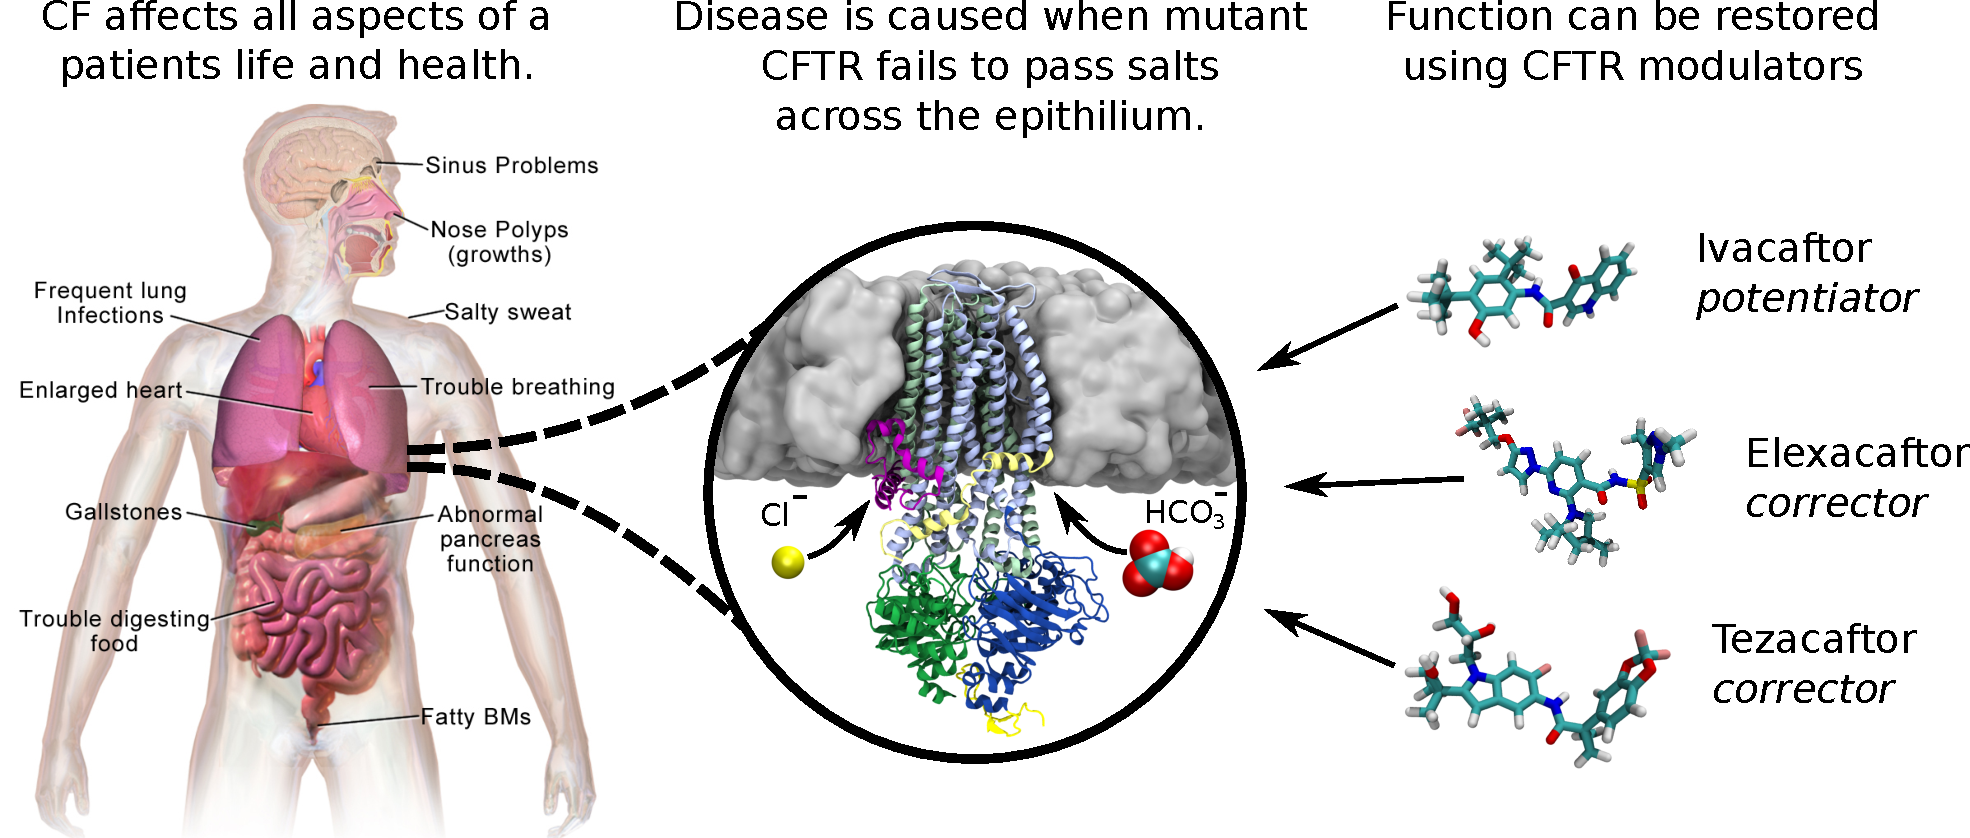
\includegraphics[width=1\textwidth]{figures/cf_summary_fig.pdf}
	\end{center}
	\captionsetup{singlelinecheck = false, justification=raggedright}
	\caption[Cystic Fibrosis is a Debilitating Disease Whose Cause is Genetic] {\textbf{Cystic Fibrosis is a Debilitating Disease Whose Cause is Genetic}}{Cystic Fibrosis causes misfunction in several major organ systems, affecting all aspects of a patients life. The cause of the disease is genetic, when two defective copies of an anion channel gene, CFTR, are inherited from each parent, epithelial cells cannot pass chloride or bicarbonate ions, leading to a pathogenic buildup of salts inside epithelial cells. In recent decades, small molecule drugs have been discovered which act directly on CFTR to restore its function. This thesis seeks to understand what kind of defects these drugs are capable of rescuing. We find that they are likely to rescue a wide range of defects.} 
\end{figure}

All organs of the body are lined by cells called epithelia. They protect organs from trauma and infection. The most acute symptoms of CF are due to the dehydration of this lining. When dehydrated, fine, motile structures on the epithelium called cilia collapse, rendering them unable to ``beat" in order to clear mucus and pathogens \cite{boucher2007, szczesniak2017}. Simultaneously, this mucus which naturally lines the epithelium is thickened as moisture is leached away from it by osmotic pressure.

This thickened mucus has pathogenic effects in several organ systems. The most acute symptoms occur in the lungs where bacterial colonies grow and form a biofilm. This damages the organ and remains one of the most troublesome chronic complications for CF patients \cite{chiappini2014}. Frequent infections mean that patients rely on antibiotics and avoid other people with CF in case they expose each other to new or drug resistant pathogens \cite{conway2008, baldoni2019}. 

In addition to these bacterial colonies, the buildup of mucus inhibits the normal function of the lungs, limiting their ability to absorb oxygen. Patients often undergo hours of physical therapy each day to help them clear this mucus from their lungs \cite{chest_pt_CFF,thefreylife2015}. Inhalation of a saline solutions may also help relieve symptoms, as this draws moisture out of the epithelial cells by counteracting the pathogenic osmotic pressure gradient \cite{wark2018}.  As figure \ref{CF_life_expectancy} indicates, much of the increased life expectancy of CF patients has been due to the improved management of this mucus and the populations of bacterium infecting it \cite{mcbennett2022}. 

In CF care, maintaining lung function remains the primary concern. The organ gradually fails over the course of the patients life, mean respiratory failure is usually the cause of death \cite{kumar2018}. The adoption of lung transplants has lead to a significant increase to the life expectancy of CF patients. However, double lung transplants remain the only option for CF patients as the CF afflicted lung left in their body would infect the donor lung with bacteria \cite{mcbennett2022}. The most common biomarker for tracking disease progress is known as FEV1\%, which stands for Forced Expiratory Volume in 1 second. It is a measure of the volume of air a patient is able to forcibly expel in one second, compared to their total lung capacity \cite{szczesniak2017}. 

CF also causes issues in the digestive system. Due to the buildup of mucus, the large intestines struggle to absorb nutrients and the pancreas cannot secrete digestive enzymes. These complications can lead to CF related diabetes which afflicts roughly half of adults with CF \cite{Kayani2018}. To manage and avoid this complication, patients are administered digestive enzymes and consume a high fat diet \cite{sullivan2017}. A patient whose pancreas does not produce sufficient enzymes to digest nutrients is referred to as ``pancreatic insufficient" (PI). This is an important determinant in the severity of disease and their quality of life \cite{halloran2011,singh2017}. 

Figure \ref{CF_life_expectancy} displays something quite interesting. As patients live longer, we must confront more disease complications. For example, once pancreatic enzymes were routinely administered, patients began to live beyond two years old \cite{roberts1957, levy2011}. This has lead to an increasing need to study and manage the role of bacterial infections in the CF lung as the increased nutrition meant they were able to fight off the infections longer \cite{burns2001}. With the advent of modulators and refinements to existing therapies, the face of the disease will change. Now that patients are living past 40 we must confront new complications such as bone disorders and infertility \cite{stalvey2013, popli2007}. This means that there still a need to study the cellular and molecular nature of CF, both its root cause and the cause of complications. 


\begin{figure}
	\label{CF_life_expectancy}
	\begin{center}
	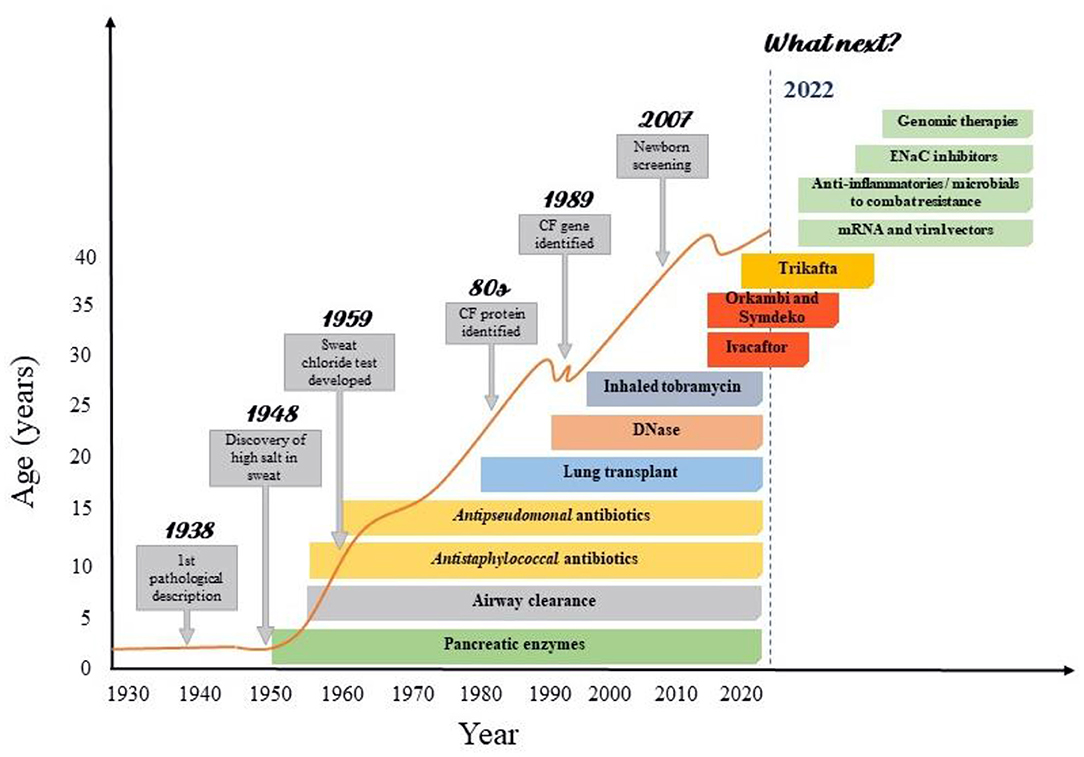
\includegraphics[width=0.7\textwidth]{figures/CF_life_expectancy.png}
	\end{center}
	\captionsetup{singlelinecheck = false, justification=raggedright}
	\caption[CF Clinical Progress] {\textbf{CF Clinical Progress}}{The orange line depicts the life expectancy of CF patients in relation to the development of different treatment. Life expectancy correlates highly with translational research. As CF becomes a chronic condition patients will likely undergo a combination of more and more advanced therapies. Source \cite{garcia2022}} 
\end{figure}


\section{The Misfunction of the CFTR Protein Causes Cystic Fibrosis}

We will now begin our journey upward, starting by understanding the molecular structure and function of the CFTR gene. From the perspective of a biophysicist, the cause of Cystic Fibrosis disease is quite simple. The imbalance of salts and water across the epithelium is due to the misfunction of a single gene---an anion channel known as CFTR.

This ion channel is unique. It is a type of protein known as an ABC transporter, designated ABCC7. The ABC super family of proteins bind ATP and use the energy from hydrolysing (breaking) ATP to pump different substrates across the cell membrane. But CFTR does not act as a transporter like the other members of its family. Rather, it can be thought of as a ``leaky pump" since it still goes through a gating cycle but is unable to actually pump substrate against a concentration gradient \cite{gadsby2006,linsdell2018}. CFTR is an \textit {ion channel}, it allows the passive diffusion of chloride and bicarbonate, but it can also pass larger anions such as glutathione (figure \ref{}) \cite{gadsby2006, tang2009,linsdell1998}. When there is not a sufficient number of functioning channels at the cell membrane, anions cannot pass out of the cell. This causes water to leach through other ion channels in order to balance this the buildup of osmotic pressure inside the cell \cite{verkman2003}. 

The evolutionary misappropriation of this protein from a transporter into an ion channel is a possible reason for why there are so many mutations which cause it to misfunction \cite{infield2021}.

\subsection{CFTR structure and function}

\begin{figure}
	\begin{center}
	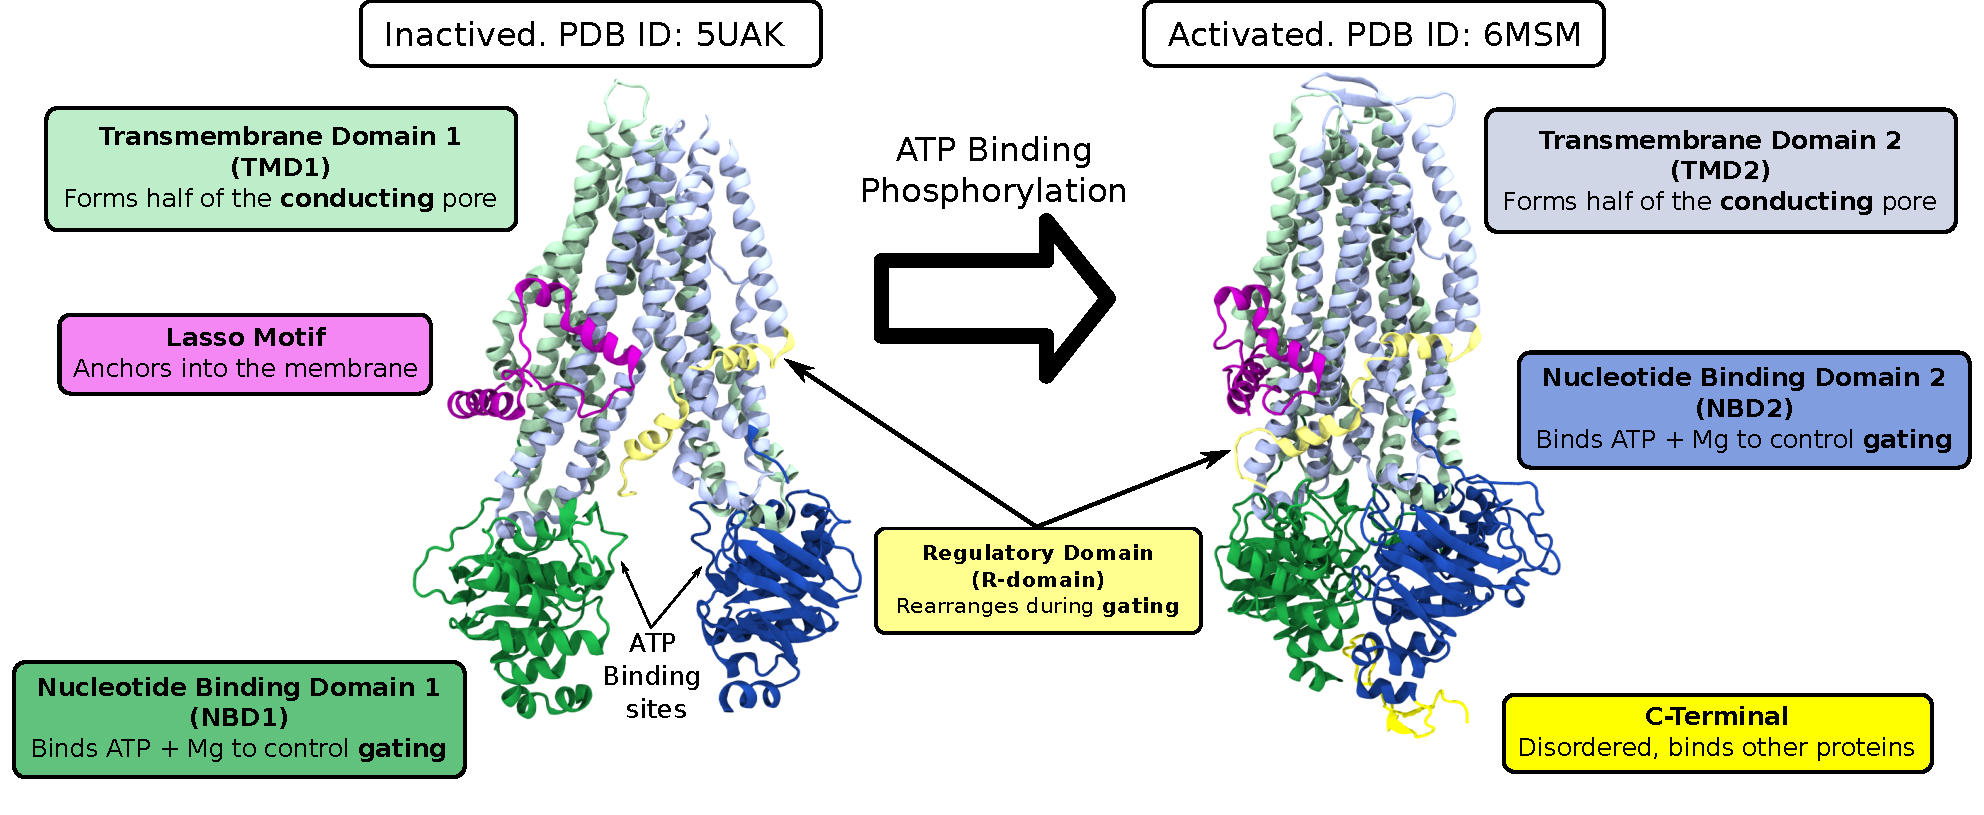
\includegraphics[width=\textwidth]{figures/CFTR_structure.pdf}
	\end{center}
	\label{CFTR_structure_domains}
	\captionsetup{singlelinecheck = false, justification=raggedright}
	\caption[CFTR Structure] {\textbf{CFTR Structure}}{There are currently two resolved human CFTR structures. The inactivated state is neither phosphorylated nor bound to ATP. Observe how the NBDs are far apart and the TMDs are not parallel, forcing a constriction near the top of the protein which does not allow the passage of ions. By contrast, the activated structure is abound to ATP at both sites, bringing the TMDs into a parallel configuration where they are able to form a pore. There are unresolved questions as to whether CFTR may conduct chloride in this conformation which we will analyse in chapter \ref{chap:opening}. All simulations presented in this work were based on the ATP-bound phosphorylated human CFTR structure. PDB ID: 6MSM \cite{zhang2018}.} 

\end{figure}
CFTR is a single chain of 1480 amino acids. The 4 main functional domains have a structure reminiscent of other ABC transporters. There  contains 

CFTR is composed of one chain with pseudo-symmetric structure, the protein is organised into 7 domains \ref{CFTR_structure_domains}. In the order of their primary structure they are: 
\begin{enumerate}
	\item The Lasso motif (AA 1-68), Which anchors into the membrane and serves as an interaction hub with protein partners such as syntaxin and filamin which are important in cellular trafficking \cite{cormet-boyaka2002, naren1998, thelin2007} as well as WNK1 which plays a role in bicarbonate selectivity \cite{kim2019}. 
	\item Transmembrane Domain 1 (TMD1, AA 69-376). This domain forms half of the chloride conducting pore and importantly, TM1 and TM6 in this domain form the extracellular end of the pore for anion permeation \cite{linsdell2006, linsdell2022}. Most positive amino acids which directly interact with anions are located in this domain, even in the inner vestibule \cite{linsdell2018}. We will look at many of these amino acids in detail in chapter \ref{chap:r352q} \cite{wong2022a}. 
	\item Nucleotide Binding Domain 1 (NBD1, AA 377-629). One of the ATP binding sites, this domain has a dense concentration of disease causing mutations, including the most common mutation $\Delta F508$ \cite{cftr2}. This domain contains a Walker A motif but lacks a Walker B motif. This causes one of the ATP binding sites to be degenerate and not allow the hydrolysis of ATP. 

	\item Regulatory Domain (R-domain, AA 630-855). A disordered domain containing up more than 11 known phosphorylation sites \cite{mihalyi2020}. In the inactivated conformation of CFTR, a helical segment of this domain wedges between the TMDs. Binding to PKA encourages this helix to unwedge from between the TMDs, while phosphorylation causes the disordered domain to remain in solution. This process has important consequences for the function of the channel \cite{ostedgaard2000, mihalyi2020}. In the open state, the wedge relocates to a location just below the lasso motif. The identity of the wedge fragment will be analysed in detail in chapter \ref{chap:I37R} \cite{wong2022}. 

	\item Transmembrane Domain 2 (TMD2, AA 856-1168). This domain forms the other half of the chloride conducting pore. There is ongoing controversy over the structure and function of TM8 the function of CFTR \cite{hegedus2022, liu2019}. This helix plays a critical role in regulating channel gating and anion selectivity \cite{negoda2019}.
	\item Nucleotide Binding Domain 2 (NBD2, AA 1169 - 1450). Home to the conserved Q-loop, which regulates the binding of ATP in ABC transporters \cite{ivey2020, zolnerciks2014, dong2015}. This domain contains both a Walker A and a Walker B motif, allowing ATP binding and hydrolysis at one of the sites. 
	\item C-terminus (AA 1451 - 1480). This structure is natively disordered but it serves as an interaction hub in WT-CFTR, anchoring CFTR to other proteins in the cell through its PDZ binding domain \cite{moyer1999, cushing2008}. 

\end{enumerate}


%CFTR is distinguished by a regulatory region known as the R-domain (residues 645-845) which links NBD1 to TMD2. This region acts to lock the channel in the closed state by wedging itself between the TMDs and dislodging when any one of 3 sites are phosphorylated \cite{mihalyi2020}. In experimentally determined structures of human CFTR the secondary structure of a section of the R-domain but not at high enough resolution to determine the identity of individual side chains \cite{zhang2018, zhang2016}. Further secondary structure information can be found through experiments with NMR \cite{Baker2007}.

Previous computational studies of CFTR have largely relied homology models based on the phosphorylated zebra fish protein PDBID:5W81 \cite{zhang2017a} or a distantly related bacterial ABC transporter SAV1866 \cite{dawson2006, Hoffmann2018}. These have yielded interesting results but the sequence similarity between human and zebra fish CFTR is only 55\%. As we will see, CFTR is highly sensitive, its function is poorly conserved under mutations. Note for example how the activity of CFTR correctors is not conserved in mutant zCFTR \cite{laselva2019}. Additionally, hte short time scales (rarely reaching 500ns) of the simulations in these studies opens the possibility that the homology model of the protein remained trapped in local minima, raising questions as to the reliability of their findings.  Hence, it is often difficult to translate the conclusions from these older studies to the human protein. 

Despite their short comings there are some studies of note which employed the use of these models. Such as \cite{belmonte2015} which used short simulation times and simple free enrgy estimates in order to demonstrate the deleterious of the G551D and dF508 mutations. This is remarkably consistent with the findings of more recent studies which can benefit from more structural information about the protein \cite{}. 

Perhaps the most interesting molecular study from this era used path-CV metadynamics to propose open state of the channel \cite{Hoffmann2018}. by combining both the zebra fish homology model and the fully outward facing conformer of SAV1866. This model has several characteristics expected of the open channel, such as the critical R117-E1124 and R352-D993 salt bridges, we will explore the latter in chapter \ref{chap:R352Q} \cite{simon2021, cui2013a}. However, it fails to create a narrow selectivity filter, which we would expect given results from \textit{in vitro} biophysical experiments \cite{linsdell2016, linsdell2017, linsdell2021, li2018b, linsdell2020, negoda2019}. However, the innovative use of metadynamics in this study did serve as the inspiration for the rigorous free energy calculations in chapter \ref{chap:opening}. 

A second study again employed metadynamics with the zebrafish structure, to study the permeation of chloride through the two extracellular portals in zCFTR \cite{farkas2020}. Unfortunately, this confirmed a difference between the zebrafish and the human structures. Experimental studies indicate that only one extracellular portal is present in the human structure \cite{linsdell2018}.

Finally, simulations of both human and zebra fish structures were used to study the stability of TM8 \cite{corradi2018}. As we will discuss in detail in chapter \ref{chap:conclusion} all CFTR structures solved by the Chen lab exhibit an unusual fold in TM8 \cite{fiedorczuk2021, liu2017, liu2019, zhang2016, zhang2018a, zhang2017a}. The helix unwinds in the middle of the membrane, a configuration that was initially thought to be energetically unfavourable. This prompted some questions surrounding the protocols used to purify and image the protein. Hence, simulations were employed in order to test whether this kinked configuration would be stable in a lipid bilayer surrounded by a solvent. It was found that the configuration of this channel was stable on microsecond timescales, with some interesting deformations introduced to the surrounding membrane \cite{corradi2018}. This indicated that the TM8 kink was indeed correct and we note that similar behaviour has been observed in our own simulations of hCFTR. Indeed, \textit{in vitro} findings would also appear consistent with this conformation of TM8 \cite{infield2021}. In particular, it was demonstrated that disulfide bridges could be  spontaneiously formed when cysteines were substituted in place of Y914 on TM8 and L102 on TM1, as other pairs of amino acids on both TM8 and TM6 \cite{negoda2019}. This stood as strong evidence that .

% , it lacks a salt bridge between R104-E116. In experiments, these residues could be replaced by cysteines and the channel would still function. However, when reducing agents were added to the system the channel lost its ability to open fully. This indicates that in the oxidised environment the C104-C116 cysteines formed a disulfide bridge but its breaking upon exposure to reducing agents caused a loss of function in the channel. This indicates that in the WT channel R104-E116 form a stable salt bridge. 

%This salt bridge is clearly visible in the recent cryo-EM structure of ATP-bound human CFTR \cite{zhang2018}.

\subsection{The Gating Cycle}

\begin{figure}
	\begin{center}
	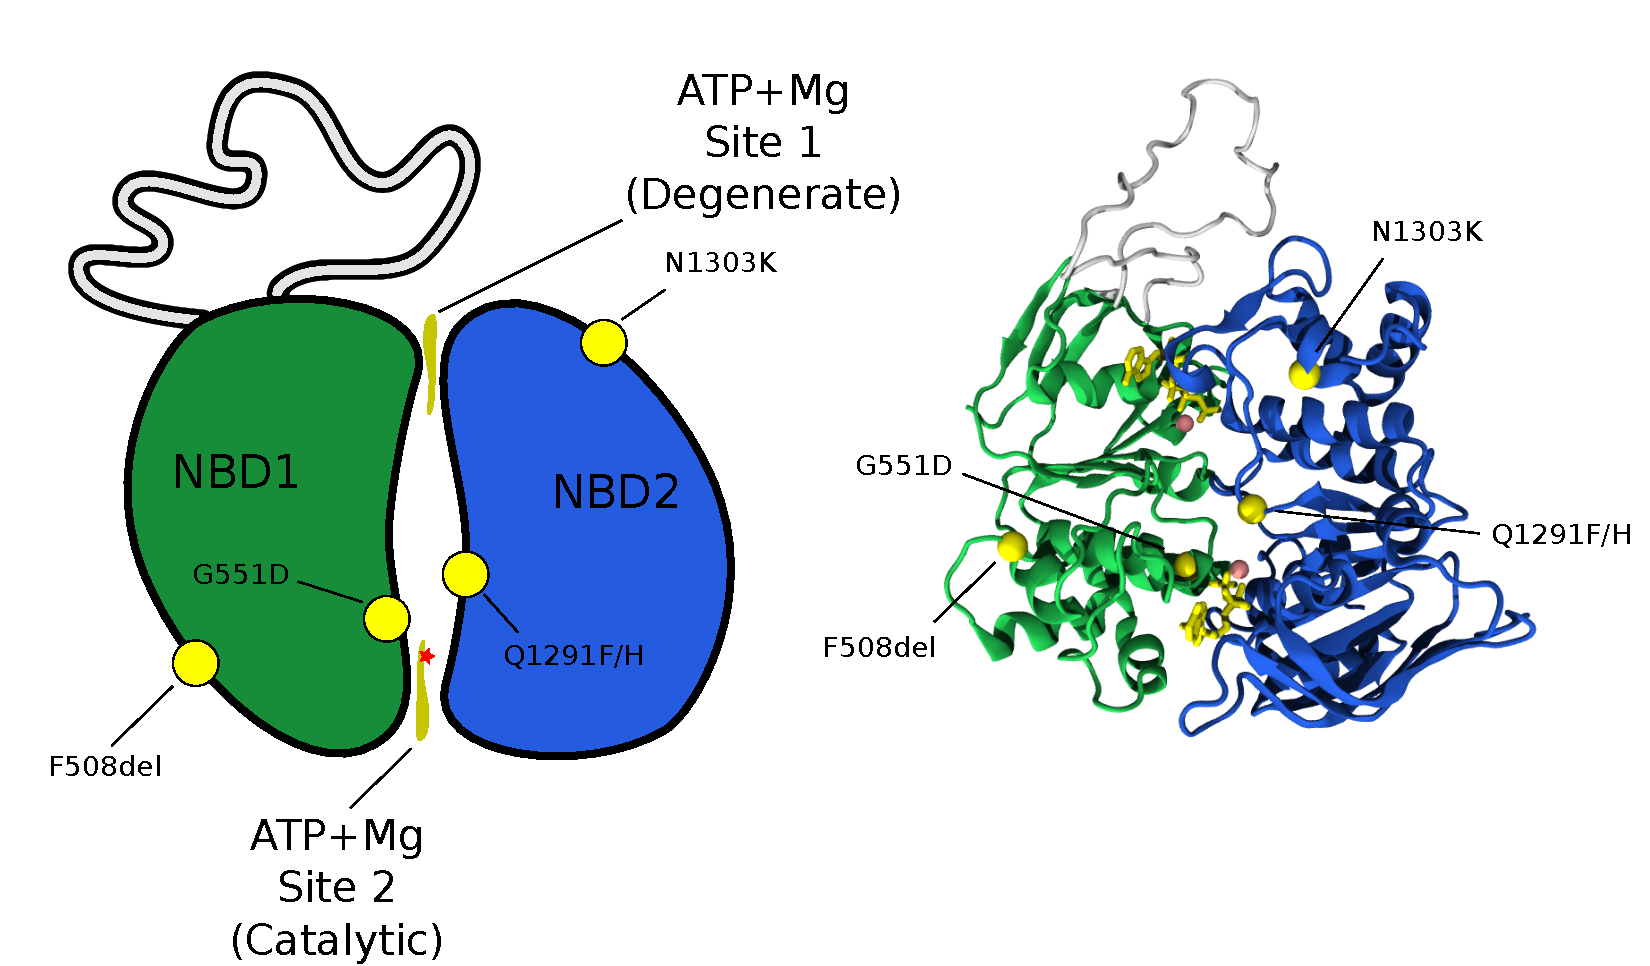
\includegraphics[width=0.8\textwidth]{figures/ATP_head_to_tail_figure.pdf}
	\end{center}
	\label{NBD_structure}
	\captionsetup{singlelinecheck = false, justification=raggedright}
	\caption[NBD Organisation] {\textbf{NBD Organization}}{A) The NBDs are critical to the gating cycle of CFTR. They rest below the TMDs where they bind and hydrolyse ATP in order to regulate the gating cycle. B) Each NBD contacts both ATP molecules. This configuration is known as a head to tail dimer and is common amongst ABC transformers. One of the unique aspects of CFTR is the fact that only one of the ATP binding sites is capable of breaking down its ATP molecule through hydrolysis \cite{stratford2007}. When ATP is hydrolysed at site 2, the channel is allowed to close \cite{infield2021}. The regulatory insertion another unique feature of CFTR and has been shown to increase NBD1 stability when deleted. The  C) Molecular details of how the NBDs bind ATP at the two binding sites. Here we have highlighted several molecular details. The Walker A motifs are on both NBDs and are responsible for stabilising ATP in a conformation which allows hydrolysis to produce ADP and a phosphate group \cite{deltoro2016}. The Walker B motif on NBD2 is directly responsible for mediating hydrolysis, by allowing the movement of the magnesium cofactor \cite{urbatsch2000, rai2006}. Mutation of E1371 in Walker B is sometimes engineered to kill catalytic activity and lock the channel in an open state \cite{stratford2007, zhang2018}. Note the placement of both G551D, a gating mutation and Q1291H/F near site 2. The most common disease causing mutation delF508 is located on a helix of NBD1 which buries itself into a hydrophobic pocket. N1303K is located at a roughly symmetric position on NBD2. } 

\end{figure}

The conformational transition from inactive to active differs significantly in CFTR compared to other ABC transporters. A transporter is characterised by acting as a gate to substrate, the substrate s never allowed to simply diffuse through. In the case of CFTR, since it is a channel the open configuration gives rise to a continuous pore \cite{linsdell2018}. The NBDs are largely similar to other to those found in other ABC transporters, they dimerise in what is termed a head to tail configuration so both subunits contact both bound ATP molecules \cite{} (Figure \ref{NBD_structure}). What is strange about CFTR is that NBD1 is missing a catalytic glutamate and so is incapable of ATP . However, the disordered R-domain is characteristic of CFTR and plays an important role in the gating cycle. Residue E1371 allows nucleophilic attack by surrounding water on the $\gamma$ phosphate  of the ATP bound to Walker B \cite{stratford2007}. The hydrolysis of ATP is the event which causes the channel to gate back to the closed conformation \cite{}. 

Read more: \cite{ramjeesingh1999}

However, the peculiarities arise from the action of the disordered R-domain. In the inactive state this wedges between the TMDs, forming a plug. Intermittently, Protein Kinase A (PKA) will bind one of many segments on the R-domain coaxing the domain into solution \cite{mihalyi2020}. PKA may then phosphorylated a section of the domain, causing to remain in an unplugged configuration. \footnote{Note to physicists, phosphorylation is a process where a phosphate group is added to the side chain of an amino acid. Usually serine, tyrosine or threonine. This phosphate group a charge of -2, wheres these amino acids are normally neutral. This is a key regulator of protein activity as it places a very large charge at a normally neutral site in the protein.}

\subsection {Anion Selectivity}

\begin{figure}
	\begin{center}
	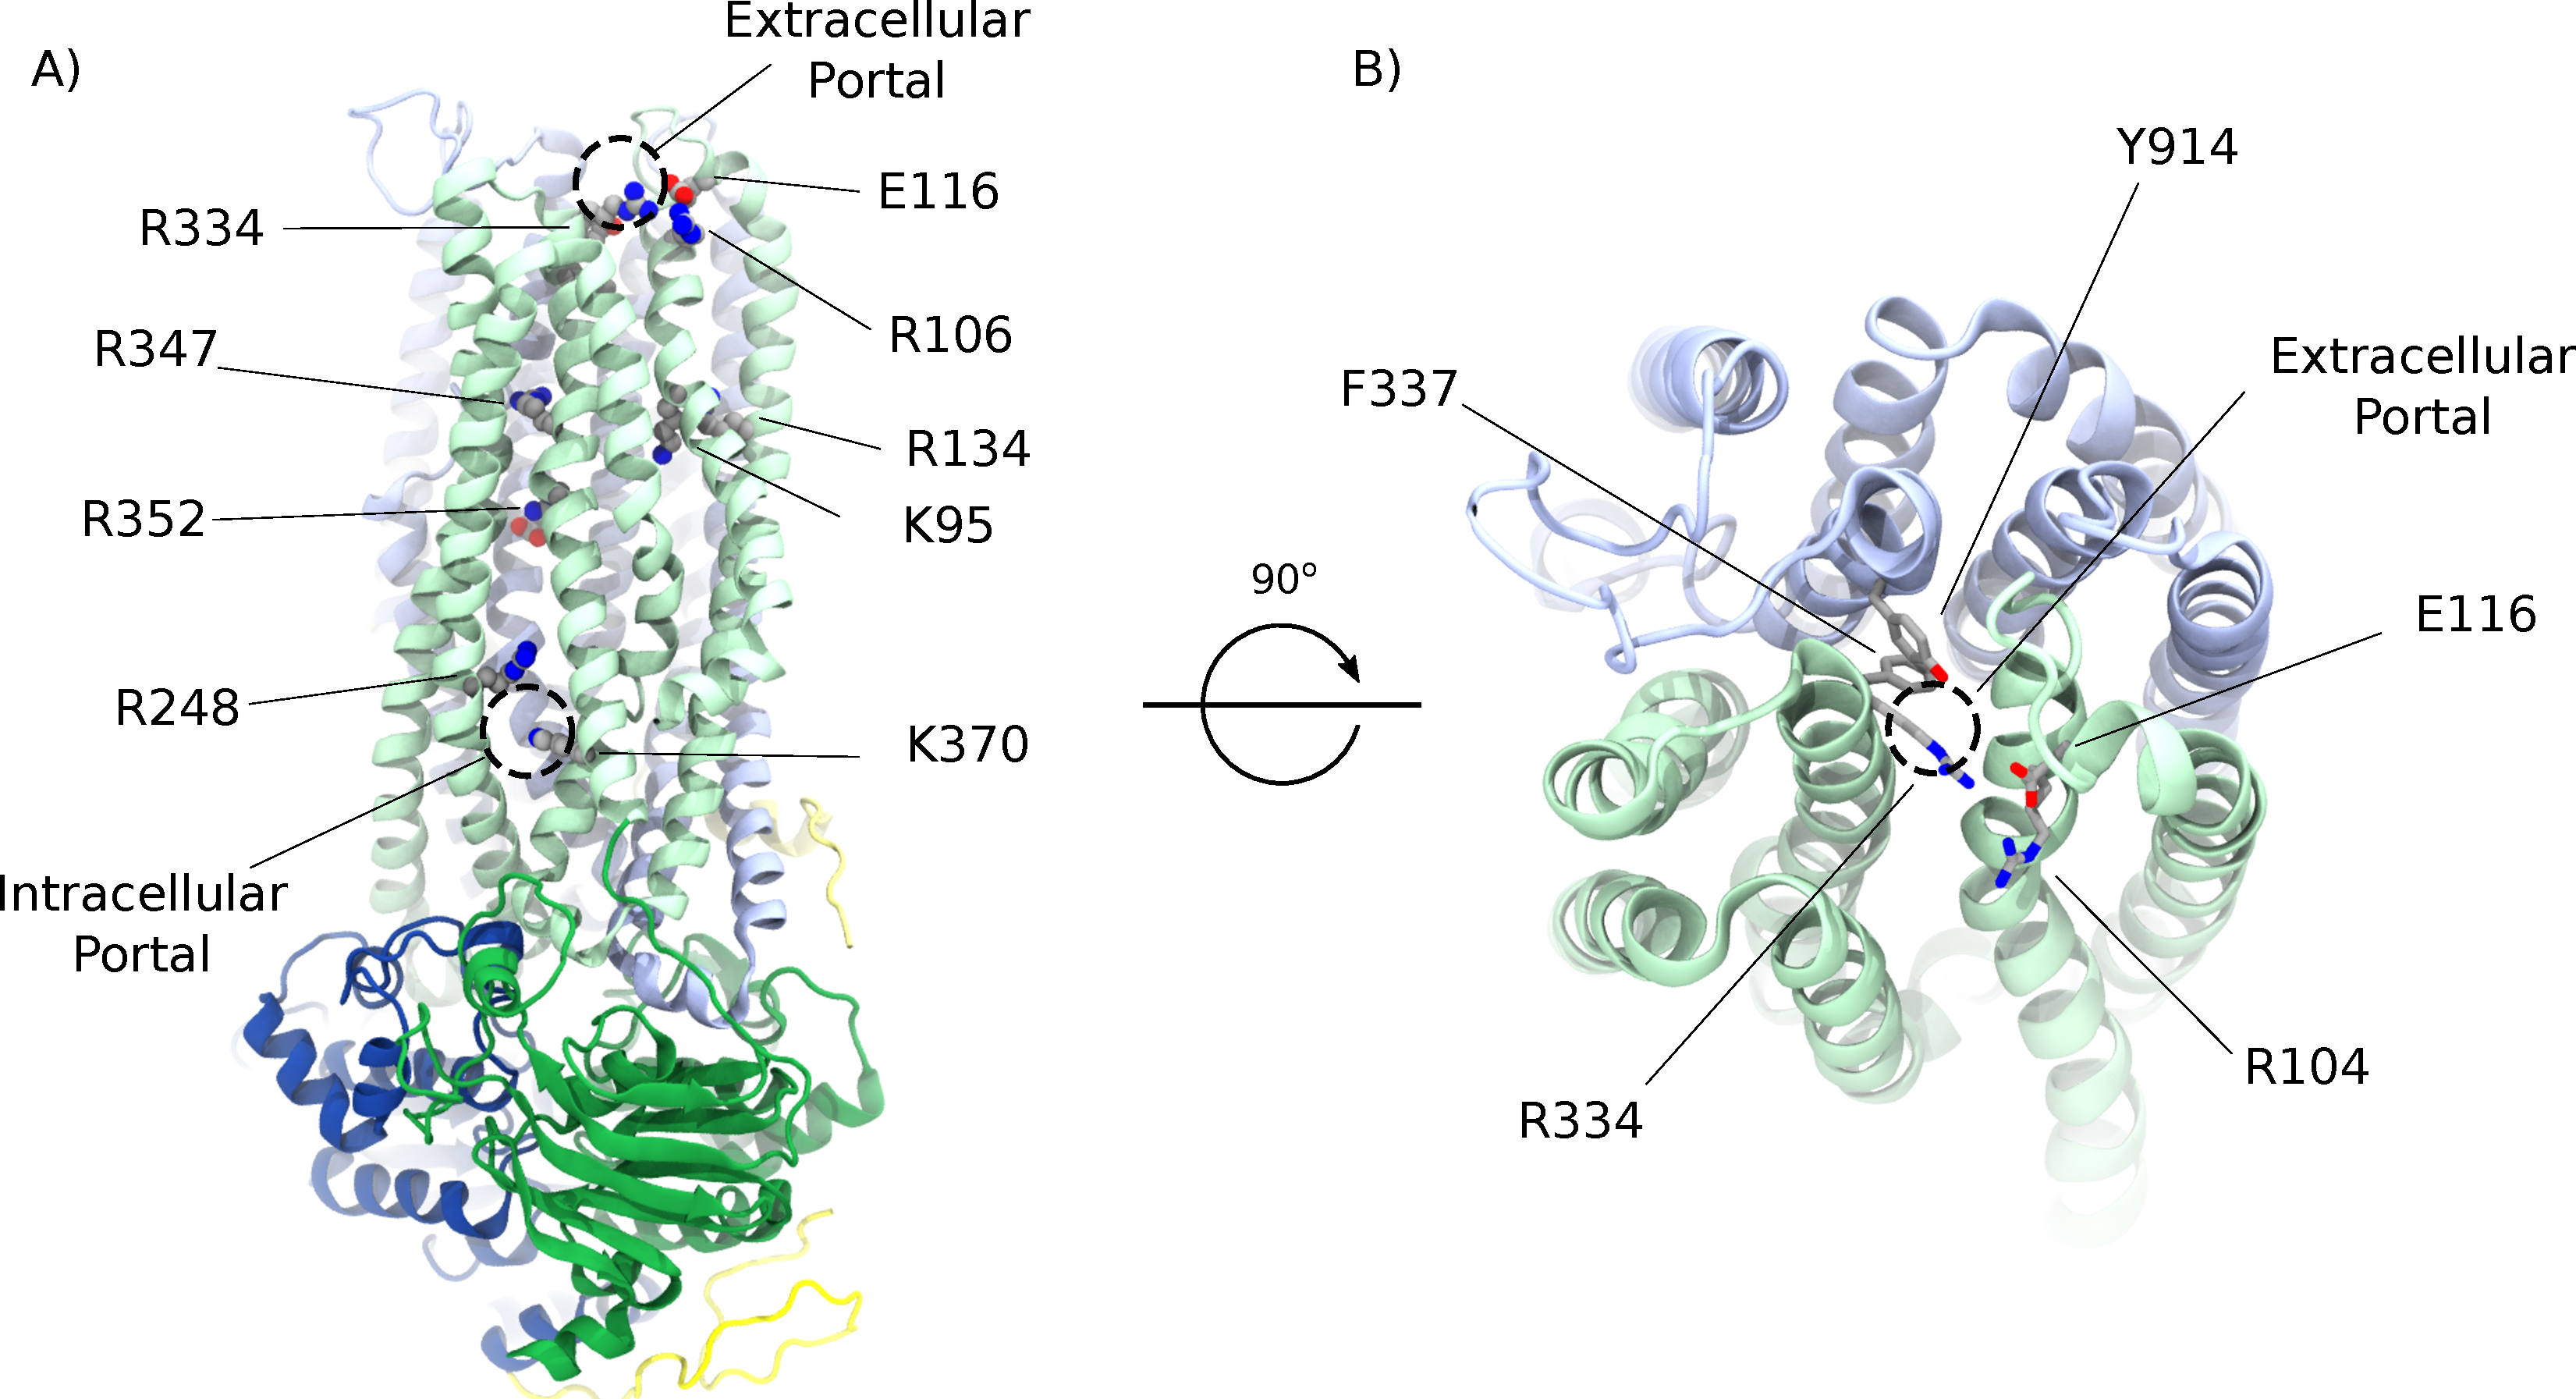
\includegraphics[width=\textwidth]{figures/chloride_passage_figure.pdf}
	\end{center}
	\label{chloride_passage}
	\captionsetup{singlelinecheck = false, justification=raggedright}
	\caption[Chlrodie Passage through CFTR] {\textbf{Chloride Passage Through CFTR}}{A)Ions enter through an intracellular gate, which is lined with positive amino acids. The subsequent inner vestibule is also lined with amino acids which chloride loosly associates with as it moves through the channel. B) A top down view of the extracellular portal. We have highlighted some hydrophobic amino acids which play important roles in the selectivity of anions. Pictured is the only available structure of the activated human CFTR channel \cite{zhang2018}. Unfortunately, this conformation is not sufficiently open to conduct ions. We will analyse an open conformation in chapter \ref{chap:opening} which we predicted through simulations.} 

\end{figure}
CFTR is weakly selective for specific anions. F337 is the most important amino acid for selectivity, with the F337A mutation leading to an increase in conductivity and a loss in selectivity \cite{wei2016}. Bicarbonate (HCO$_3^-$ is known to have roughly 26\% the permeability of chloride through the channel. An interaction partner WNK1 has been shown to influence the selectivity of the channel https://www.ncbi.nlm.nih.gov/pmc/articles/PMC6889609/. The permeation of bicarbonate is very important physiologically because if a mutation permeates bicarbonate it means there is a high likelihood the patient will be pancreatic sufficient. This is being explored as a possible therapeutic strategy \cite{ferrera2021}. 

Compared to cation channels like Gramicidin and KcsA, CFTR is only weakly selective, permeating a large set of anions with varying radii and geometries \cite{}. Supposedly it is more permeant to lyotropic (low solvation energy anions) rather than cosmotropic anions (high solvation energy anions) indicating that dehydration of the anion is likely during conductance (CITATION NEEDED). The radius of hydrated chloride ions is 1.7A \cite{yang2002} so even with this larger pore partial dehydration must take place. 

Molecular dynamics studies of the conductance of chloride through the 6MSM structure only saw one extracellular portal. However, they observed multiple pathways between helices. Only 17 conduction events were observed in 10 microseconds of sampling, with a substantial bias of 500mV. This is an order of magnitude less than we would expect for the 0.7 $10^{-12}$S conductance channel. When we consider that the channel must also pass diverse substrates such as bicarbonate, iodide and glutathione, we would expect a more open conformation to exist \cite{kogan2003,linsdell1998}. Such a discrepancy was the basis for the studies in chapter \ref{chap:opening}.


\subsection{Different classes of Cystic Fibrosis Phenotype}
The more than 400 disease causing mutations to CFTR have been classified into 6 common classes based on the nature of the CF they cause, their reaction to CFTR modulators, and results \textit{in vitro} assays. Ultimately I aim to show that at the atomic level there is much more nuance to these and as patient specific theratyping evolves, these classes will become less relevant, serving as illustrative tools only to communicate at a higher level what is going wrong with the CFTR protein. The canonical classification is as follows:

\begin{figure}
	\begin{center}
	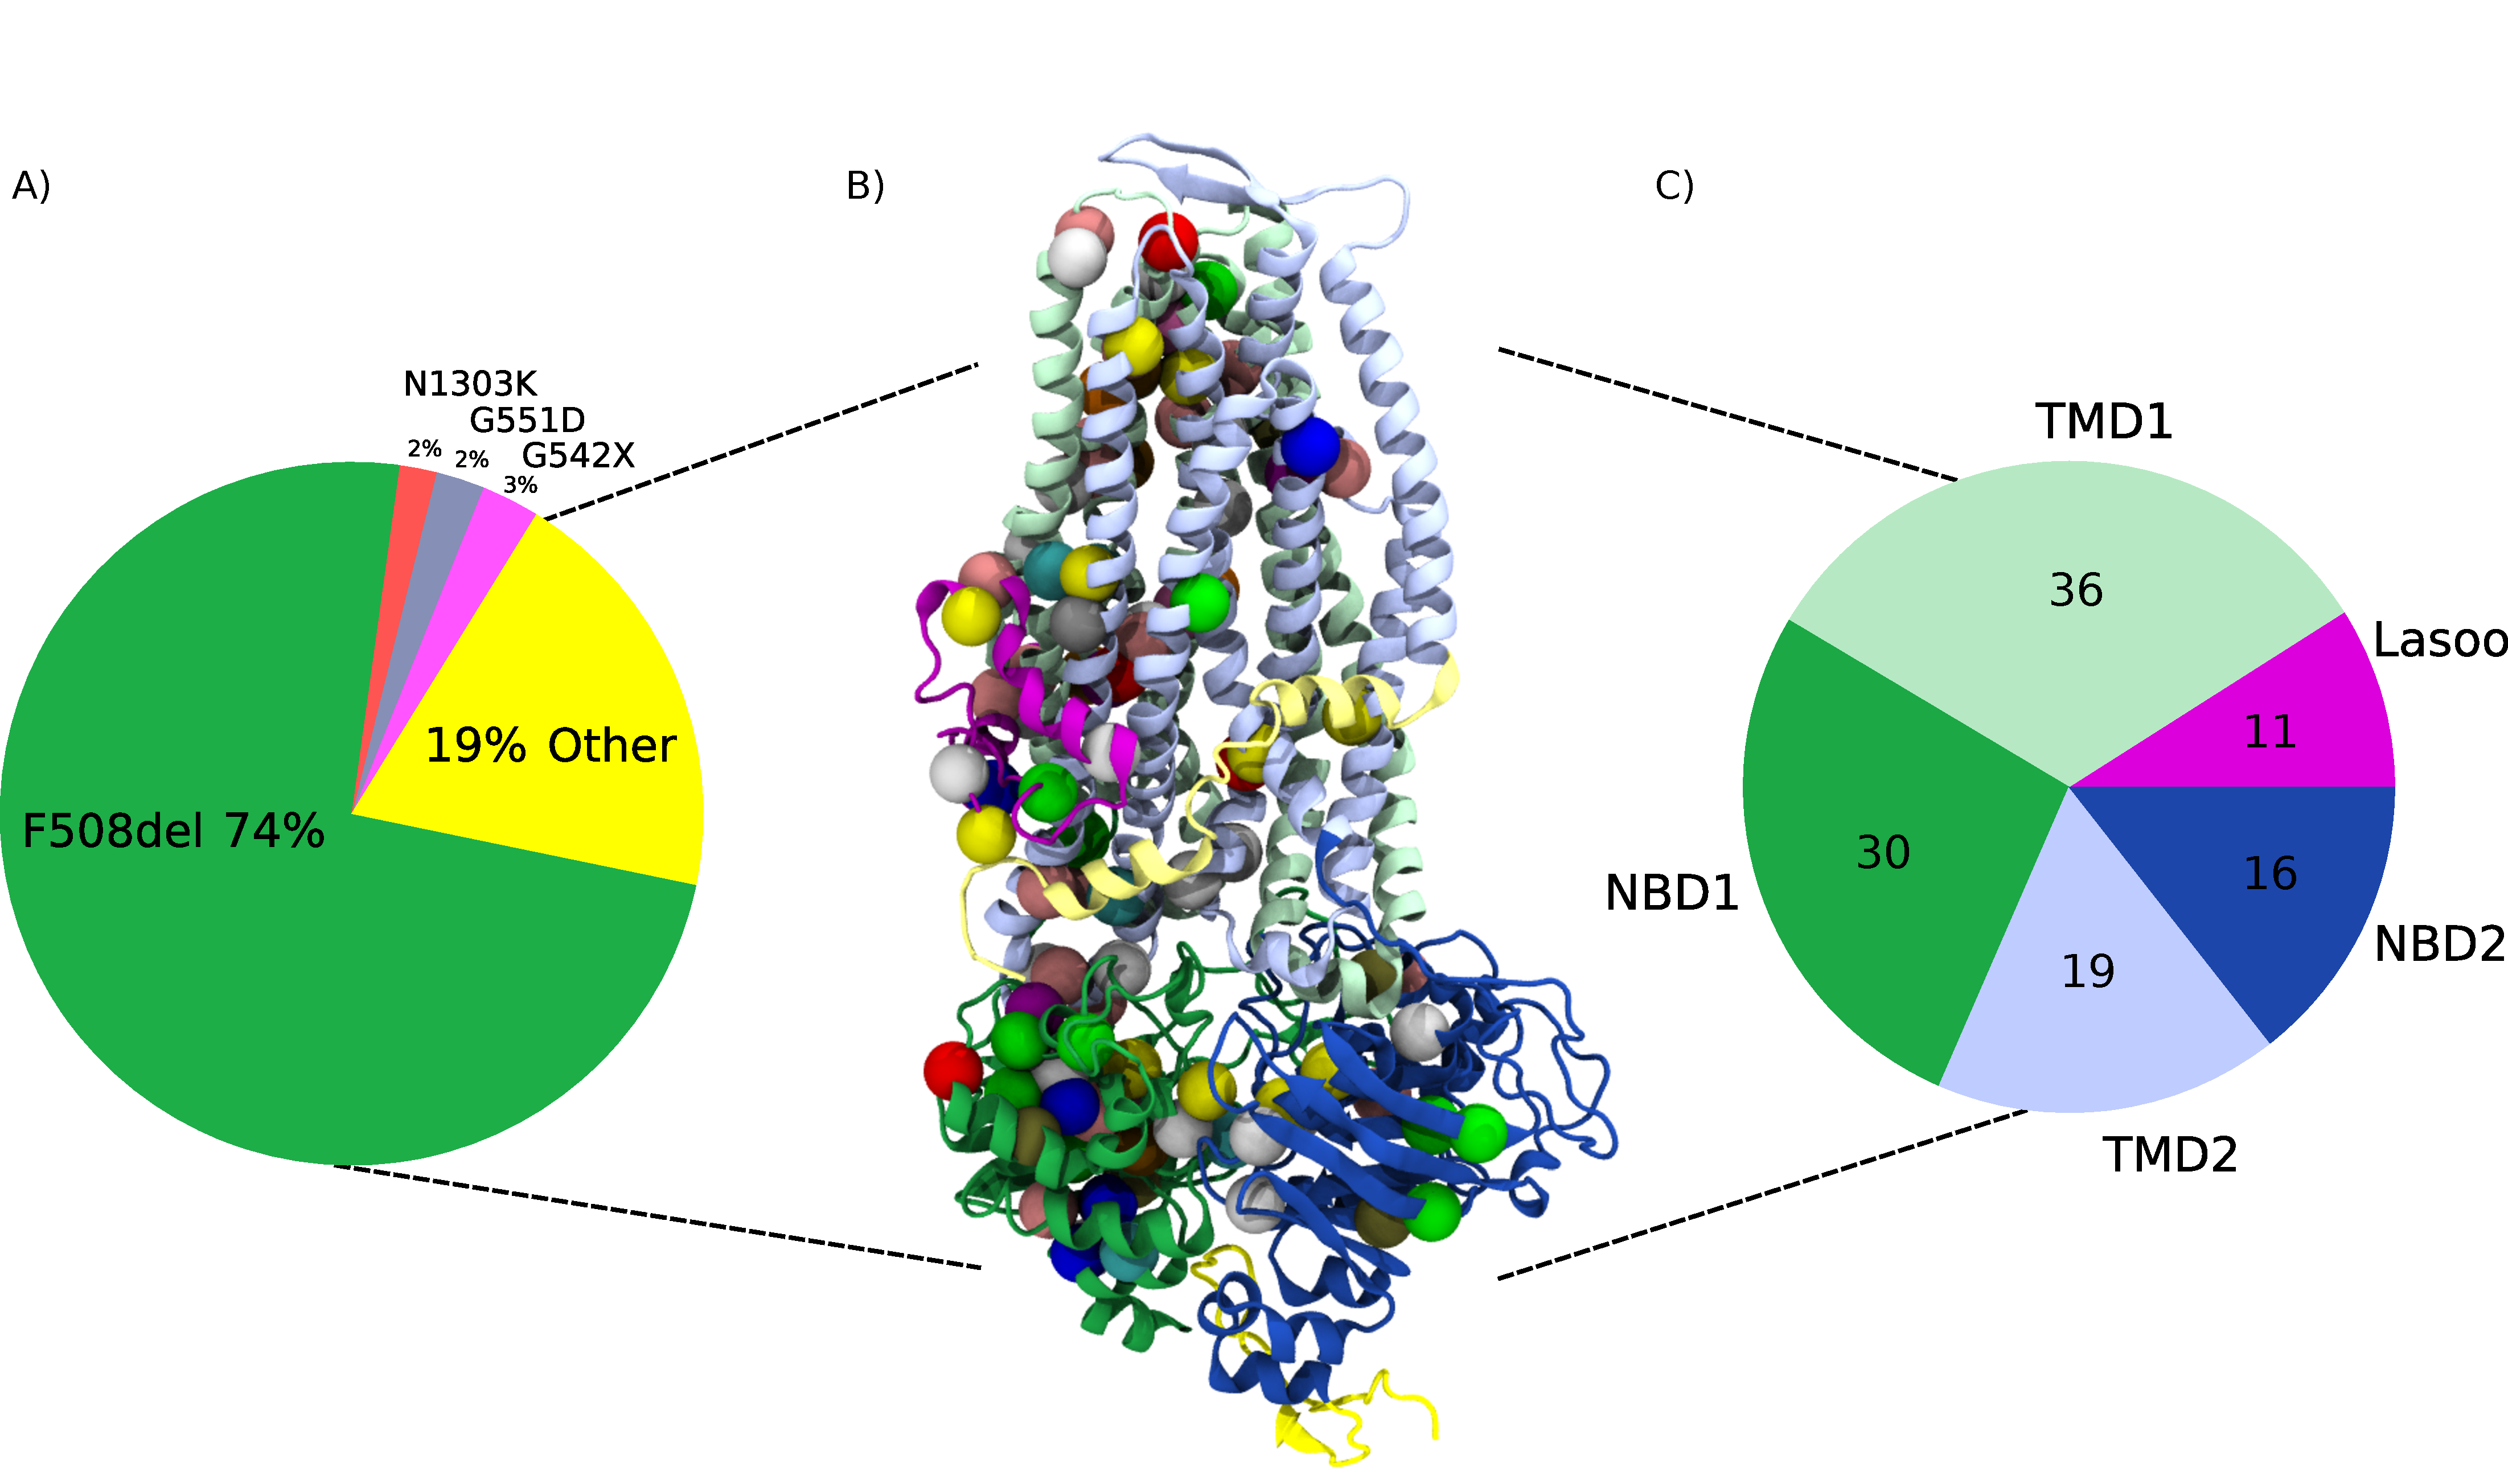
\includegraphics[width=\textwidth]{figures/alleles_pie_chart.pdf}
	\end{center}
	\label{CFTR_structure_domains}
	\captionsetup{singlelinecheck = false, justification=raggedright}
	\caption[Rare Mutations Occur in Across the CFTR Protein] {\textbf{Rare Mutations Occur in All parts of the CFTR Protein}}{A) The reported frequency of all disease causing alleles (not just missense mutations) in the CFTR2 database. At the time of writing there are 402 recorded different disease causing mujtations. A patient with CF will carry two of these mutations. 1 in 25 people of Northern European descent are a carrier for CF and are themselves at increased risk for many health problems \cite{ioannou2014, miller2020}. B) The location of all 112 known disease causing missense mutations mapped on the CFTR protein itself as spheres. In addition to those visualised here there are many of variants of unknown significance (VUS) which may cause disease but are so rare they have not been clinically studied. C) The incidence of CF causing missense mutations in the different domains of the CFTR protein. TMD1 and NBD1 have the highest concentration of disease causing mutations. Likely due to the former's role in ion permeation and the latter's role in gating \cite{cftr2}}. There are no confirmed CF causing missense mutations in the C-terminus or the R-domain. As patient registries are set up across the world it is likely that more rare CF causing mutations will be discovered in the future. \footnote{Note that in this figure we have included the novel I37R mutation studied in this thesis. This mutation has not yet been recorded in CFTR2.} 
\end{figure}


\begin{itemize}
	\item \textbf{Class I} No functional protein. Under these mutations no protein is transcribed due to either problems with the transcription of mRNA or a premature stop codon truncating protein synthesis early, meaning the resulting peptide is missing key domains. 
	\item \textbf{Class II} Folding defect. These mutations cause the translated peptide to misfold into the incorrect tertiary structure. This can inhibit the protein's journey as it is trafficked to the cell membrane. 
	\item \textbf{Class III} Impaired Gating. Here the mutation inhibits the ability of the protein to transition from the closed to the open state. 
	\item \textbf{Class IV} Decreased Conductance. These mutations cause a barrier in the energy landscape of the CFTR chloride conductance pathway.
	\item \textbf{Class V} Less Protein Expressed.  
	\item \textbf{Class VI} Decreased Functional Lifetime

\end{itemize}

Although useful from a clinical and experimental standpoint, in reality these classes do not reflect that a mutation may belong to many categories at once, to differing degrees. This has lead to a more granular approach to the classification of mutation phenotypes in more recent studies \cite{veit2016}. In particular in this thesis we will demonstrate that membership of one of these classes can be due to a range of molecular phenotypes. Hence, this classification is becoming increasingly outdated and there is a need to understand the unique overlapping molecular phenotypes of each mutation. Further, through our molecular simulations we will see that in fact CFTR modulators appear capable of treating many different mutations with unique modes of pathogenesis. We will explain this paradigm in more molecular detail in chapter \ref{chap:conclusion}.

%FIGURE demonstrates how each of the canonical classes at the molecular level is broken down into many sub classes and a mutation might belong to one of many of these subclasses. Structural biology paradigms and \textit{in silico} modelling can help classify mutations into these different classes. In combination with wet lab assays we can understand which classes of these molecular defects are most effectively treated with specific drug regimens. Our computational microscope is helping choose treatments for patients at the atomic level. 

\section{Modulators Act Directly on CFTR to Restore its Function}
\begin{figure}
	\label{drugs_bound}
	\begin{center}
		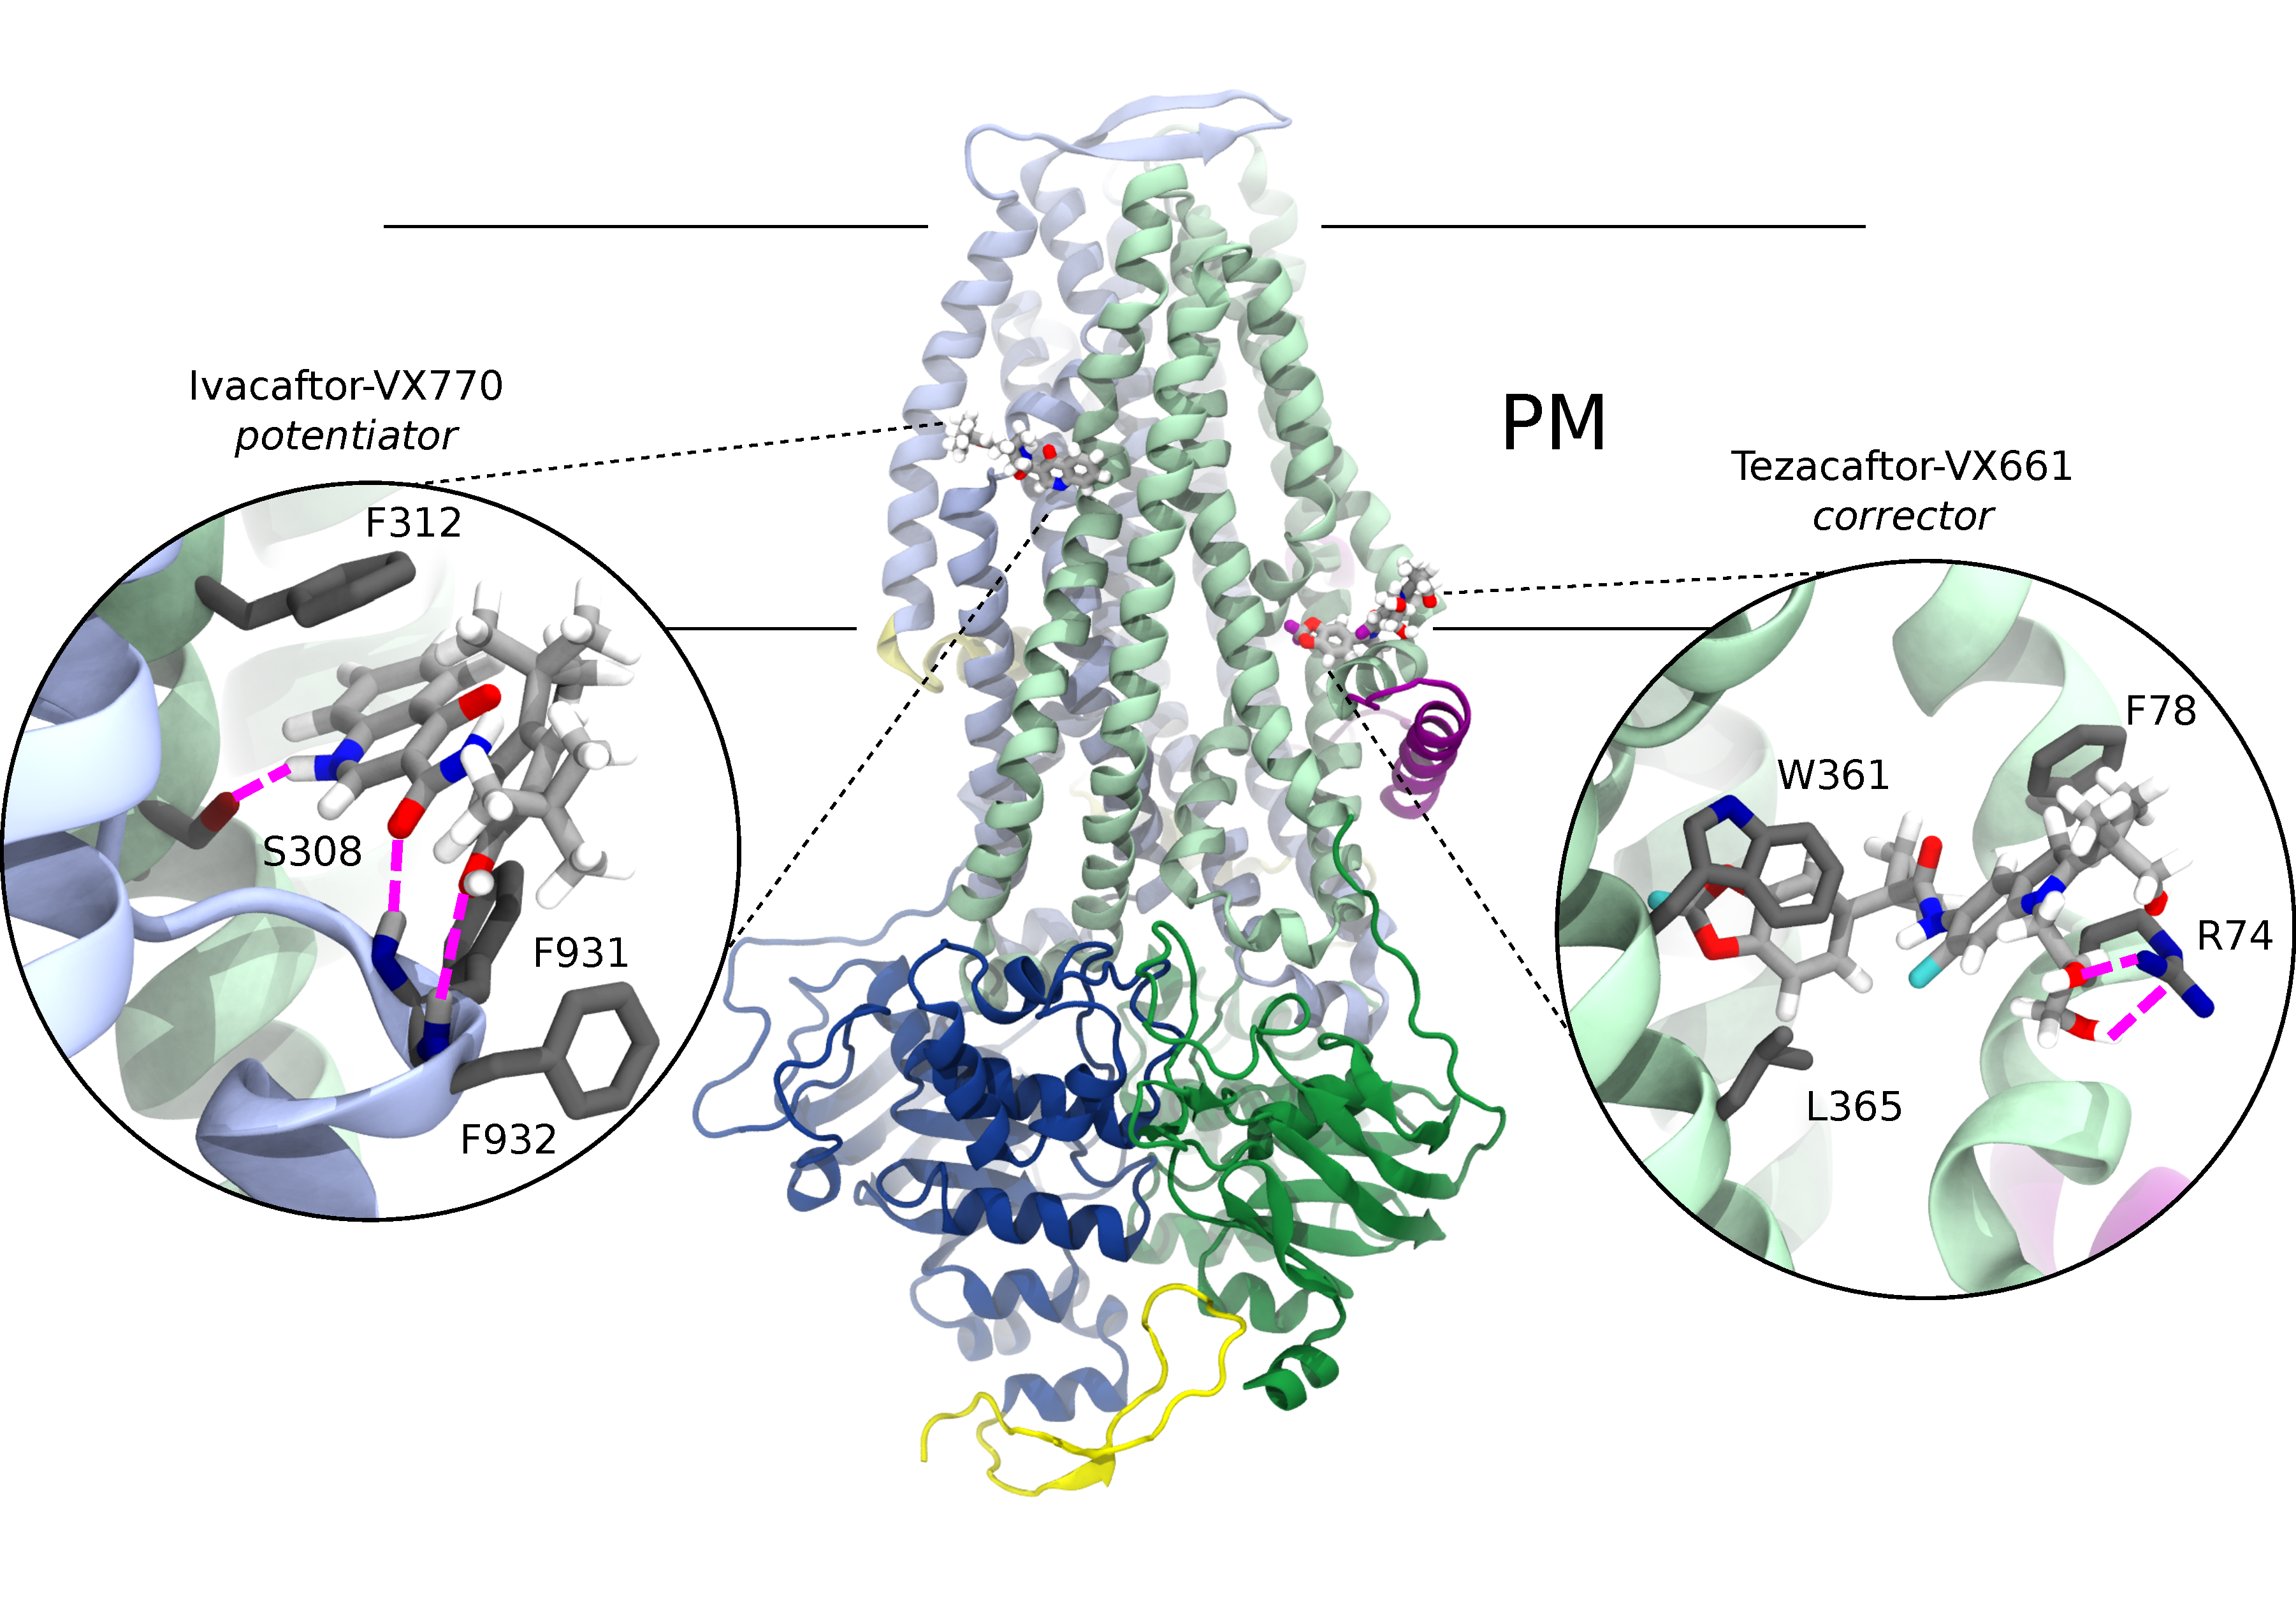
\includegraphics[width=1\textwidth]{figures/drugs_bound_overall.pdf}
	\end{center}
	\captionsetup{singlelinecheck = false, justification=raggedright}
	\caption[Modulators Bound to CFTR] {\textbf{Modulators Bound to CFTR}}{The structurally imaged binding sites of potentiators and class 1 correctors \cite{liu2019, fiedorczuk2022}. Potentiators in particular are proposed to bind to other sites as well \cite{yeh2019, liu2019}. Hydrogen bonds are labelled with purple dotted lines. Note how both visualised binding sites require substantial contributions from the surrounding lipid bilayer. The presence of these lipids will play an important role in the binding kinetics and energetics of these drugs \cite{csanady2019}. Future molecular studies should account for these nuances.} 
\end{figure}

Since CF is caused by malfunctions of CFTR, it has been pursued as an attractive target for drugs. Through high throughput \textit{in vitro} screening four compounds which act directly on CFTR have been clinically aproved for the treatment of CF. These drugs fall into two classes. Correctors, which aid CFTR to fold into the correct state and potentiators which help the channel reach the fully open state once it has folded correctly and integrated into the membrane. Subtleties surrounding the high affinity action of potentiator drugs opens the possibility that specific genetic defects may be optimally rescued by specific combinations and doses of both correctors and potentiators compounds \cite{csanady2019}. Recently, cryo-EM structures of many of these compounds in their bound state have been published \cite{liu2019, fiedorczuk2022}. In addition to several \textit {in vitro} biophysical experiments to determine the precise mechanism of action and binding site of these compounds \cite{csanady2019,  }.

What is remarkable is that modulators they have demonstrated promise in improving not just the most acute symptoms of CF (lung function), but they may be able to treating or even relieve deleterious complications. Modulators have been found to relieve pancreatic insufficiency and CF related diabetes symptoms \cite{gaines2021,lopes-pacheco2020, yi2021} and there is ongoing ongoing study into the possible benefits of modulators on bacterial infections \cite{harvey2022}. This highlights the importance of treating the root cause of a disease like CF.

\subsection{Correctors}
Corrector class modulators are able to treat Class II folding defects. They appear to help the CFTR protein fold into the correct structure by binding to a pocket formed between TM1 and TM3. This hypothesis was generated from circular dichromism \cite{greenfield2006} and fluorescence experiments found that an isolated construct of TMH3 and TMH4 were more likely to fold correctly in the presence of corrector compounds. Later, cryo-EM structures were able to directly image the drugs bound in this location, confirming this hypothesis \cite{fiedorczuk2022}. 

In combination this is strong evidence for the precise mechanism of action for corrector compounds. Further work will aid in the creation of new compounds to refine our exploitation of this mechanism.

\subsection{Potentiators}
Potentiator class drugs bind to CFTR in order to increase the population of conducting channels,  helping to balance osmotic pressure over the epithelium \cite{jih2013,yeh2017}. 

There is some uncertainty surrounding the molecular details surrounding the mechanism of potentiators drugs, with different studies discovering different binding sites via mutagenesis and other methods \cite{yeh2019, liu2019, laselva2021}. Evidence strongly supports their findings that potentiators bind directly directly to CFTR in order to increase the likelihood that it occupies a conducting state, with some potentiators rescuing CFTR with picomolar affinity \cite{csanady2019}. The controversy arises surrounding precisely \textit{where} these drugs are binding in order to rescue CFTR. There are are cryo-EM structures which show the drugs bound to the TM8 hinge region which is itself controversial due to its unique conformation \cite{liu2019}. We will address these controversies in more detail in chapter \ref{chap:conclusion}. \textit {In vitro} experiments studying drug binding kinetics suggest at least two membrane facing binding pockets \cite{csanady2019}. 

GLPG1837 has not been approved in a clinical setting. \textit {In vitro} experiments suggest that it is more efficacious even though it has lower affinity for CFTR binding \cite{vanderplas2018}. This would indicate that the highest affinity binding pocket does not produce the greatest modulation. More work is needed to resolve the mechanism which results in the highest clinical effectiveness of these drugs.  

In our work we've found that the atomic nature of the defects introduced by each mutation varies widely, what is interesting is that experiments in \textit{ex vivo} have shown that these drugs are still able to treat this range of different defects. The classification of classes of defect is outdated, really there are as many classes as there are mutations.

\subsection{Future Therapeutic Strategies}
\subsubsection{Read Through Compounds}
Roughly 10\% of mutations result in a premature stop codon in the mRNA of the CFTR gene so synthesis is stopped early. Since there is no full length CFTR protein synthesised by the cells carrying this mutation, potentiators and correctors are unable to directly assist. This has lead to the need to develop a class of drugs known as read through compounds which allow the continued synthesis of the protein past the premature stop codon \cite{sharma2021}. At the time of writing no read through compounds have been clinically approved but efficacy has been demonstrated in pre-clinical models\cite{crawford2021}. Since correctors and potentiators also modulate the behaviour of WT-CFTR it is likely that correctors and potentiators would be given in combination with read through compounds and other therapies as a Complimentary treatment.

\subsubsection{Alternative Strategies}
As the root cause of disease, CFTR will continue to be an important therapeutic target. However, there will also be increasing value in the therapeutic benefit derived from manipulating other protein systems---both as complimentary a strategy to the modulation of CFTR and to the treatment of complications. This is especially pertinent when we consider that some patients do not respond to CFTR modulators, even when they share the genotype of patients who do. These patients would benefit greatly from complimentary therapeutics \cite{hanafin2021, robertson2015, lingam2017, seelig2020, barbieri2021a, grebert2019}. 

\section{Patients with Rare Mutations Struggle to Access Modulator Therapy}
CFTR modulators have proven to be a breakthrough in the treatment of CF. However, there is strong motivation behind our focus on rare mutations in this thesis. Roughly 50\% of Cystic Fibrosis cases are caused by a homozygous mutation, $\Delta$F508, and 90\% of patients carry at least one copy of this mutation. At the time of writing, many jurisdictions such as Australia and the EU have approved a triple therapy known as Trikafta which can improve the outcomes for patients with one copy of $\Delta$F508. However, this leaves a significant part of the CF afflicted population without access to this life saving medication, with many more excluded due to the extreme cost of the drugs themselves \cite{administration2021, trikafta_website, abdallah2021, guo2022a}. Clinical studies are also extremely difficult for rare mutations, as there may not be enough patients carrying a specific mutation to study them in the same trial \cite{grody2007}. The work in this thesis demonstrates that a larger section of the CF population is likely to respond to modulators, particularly those carrying missense mutations. Eventually this work will contribute to a clinical method known as theratyping. An increasingly granular understanding of CF pathogenesis will allow a personalised choice of treatment.

The treatment of rare mutations has particular significance in CF. Not only would patients be otherwise left behind, but by studying rare mutations, outcomes can be improved for all sufferers of CF. For example, potentiator class drugs were discovered by the study of the rare mutation G551D, through high throughput molecular screening \cite{vangoor2009}. By studying rare mutations we can gain a more complete understanding of the nature of the disease and so improve therapies for everybody. This approach will become more important in the future as CF is uncovered in regions where it is rarer, and the population exhibits a broader spectrum of CFTR mutations. Patients in these regions are thus more likely to have a rare form of disease \cite{singh2015,zheng2017,ni2022}. As patient registries are set up in these populations, more rare forms of CF are likely to be discovered \cite{zheng2017}. Considering that patients with the same genotypes often respond differently to the same modulators, it is critical that more modulators are developed, to give all patients more options and better outcomes \cite{hanafin2021}.

%Patients with rare forms of CF are more likely to be in countries where CF is already quite rare \cite{zheng2017}. Patients on modulators have significantly different clinical outcomes even between those with the same genotype. Determining the reason for this would open the door to the development of complimentary therapeutics. 

By explicitly focussing on rare mutations in this thesis we aim to prove that a large subsection of the CF community currently excluded from receiving modulator may in fact to respond to modulators therapy. It would seem that CFTR modulators are capable of treating a wide range of molecular defects. All of the mutations studied in this thesis have a unique mode of pathogenesis but they appear to respond to existing modulators with the same mechanism of action. Such an approach is critical as the earlier patients are able to start modulator therapy the better their prognosis \cite{lahiri2022}. The drugs are well tested in terms of safety and efficacy and now we aim to expand the number of patients who can access modulator therapy \cite{lahiri2022}.

\section{Patient Derived Organoids: A Pre-Clinical Model to Assess Modulators}
Similar to how we calculated the motions of interacting atoms in chapter \ref{chap:methods} to model a whole protein system, medical researchers seek to would also like to find a model system to study the function of an organ. In CF research, this has lead to the development of techniques where samples of epithelial stem cells from patients the disease are grown into tissues which mimic the function of either the lung or the gut \cite{wong2015,depoel2020}. This is possible in the due to a population of adult stem cells in the epithelium which maintain the ability to differentiate into a variety of cell types (a property known as pluripotency) \cite{blanpain2007}. 

Primarily, these epithelial stem cells are taken from the nasal passages, in order to grow lung organoids of patients or from rectal biopsies which can be grown into intestinal organoids \cite{awatade2021,sato2011}. The morphology of the organoids can be confirmed through immunofluorescence microscopy \cite{awatade2021, im2019}. Organoids are excellent model systems, but we should note that like all models they are incomplete. They often lack specialized cell types and miss much of the complexity of native organs \cite{clevers2016}. 

However, these models are emerging as an excellent surrogate for clinical trials, overcoming a complex, time consuming process \cite{pranke2019a} which might usually be inaccessible to patients with rare and ultrarare mutations. 

Adult stem cells in the epithelium are preferable to other sources of stem cells, as sources which might be easier to harvest such as iPSCs from the skin or white blood cells would require complex, time consuming protocols to grow into organoids \cite{wong2012}. Already, the differentiation and expansion of epithelial samples into the organoids studied here takes one month \cite{sato2011}.

In the case of CF, this technology allows the construction of a scalable, patient specific platform where a patient's own tissues can be tested to determine the best treatment for them \cite{keegan2021, sato2011}. These pre-clinical models will allow more patients in the heterogeneous set of disease causing mutations to access modulators. This has given rise to an exciting prospect of a practice known as theratyping, enabling clinicians to make a personalised prediction of which therapies will best serve a patient \cite{clancy2019, wong2022, wong2022a, ciciriello2022}. This thesis demonstrates that integration of \textit{in silico} simulations into the process of theratyping can further the capabilities of these pre-clinical models.

%One limitation of these organoid platforms is the lack of an inflammatory response since no immune cells are present in the tissue culture. 
Subsequent chapters will make use of these organoids by testing them with a set of \textit{in vitro} assays in order to characterise a patient's response to modulator therapy, so they are discussed briefly below.

\subsection{Forskolin Induced Swelling to Assess CFTR Function}

\begin{figure}
	\label{western_blot}
	\begin{center}
	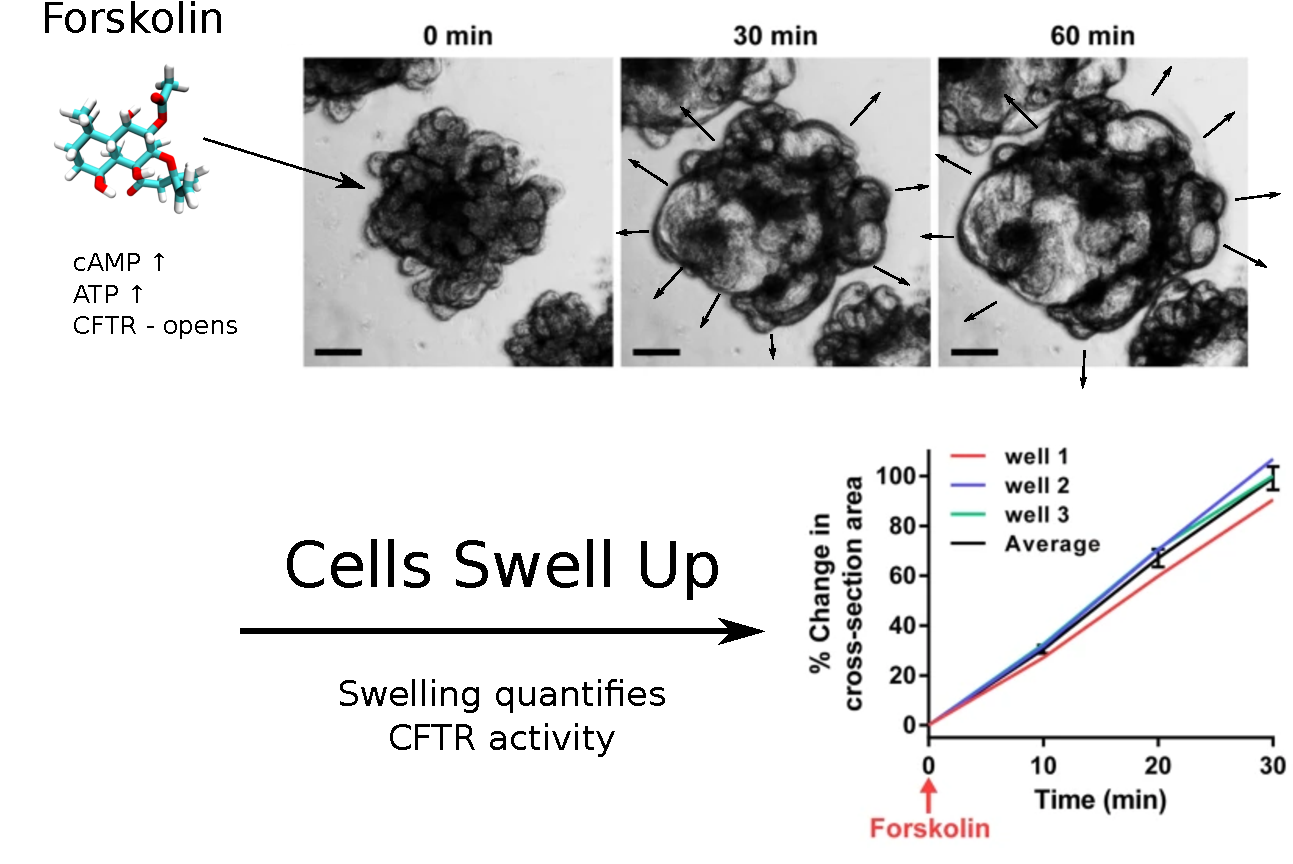
\includegraphics[width=1\textwidth]{figures/FIS_demo.pdf}
	\end{center}
	\captionsetup{singlelinecheck = false, justification=raggedright}
	\caption[Forskolin Induced Swelling] {\textbf{Forskolin Induced Swelling}}{Upon exposure to Forskolin, epithelial cells begin to produce cAMP. This causes an increase in intracellular ATP which will open CFTR channels. The influx of water into the cell causes them to swell. The amount of swelling can be used to quantify the amount of properly functioning CFTR in the cell.} 
\end{figure}
Forskolin Induced Swelling (FIS) assays have been used to characterise the patient specific response of a patient's organoids to a drug regimen \cite{dekkers2013}. When epithelial cells are exposed to a chemical known as Forskolin they begin to rapidly produce cyclic AMP (cAMP, a precursor to ATP in a cell) \cite{bonora2012}. The presence of ATP activates the CFTR ion channels, causing the organoids themselves to swell. This swelling allows cell biologists to easily quantify the activity of CFTR within a cell in a variety of conditions, such as the presence of drugs.

\subsection{Electrophysiology Directly Measures CFTR Gating and Conduction}
Since CFTR is an ion channel, measuring its electrical activity is a direct way to assess its function and dynamics. For single channel studies this is done with a patch clamp. However, this does not give an assessment of the whole epithelium. Often the whole organoid is used as a patch and put in an Ussing chamber. By blocking other ion channels such as ENaC during measurements, \footnote{ENaC inhibitors are also being explored as a complimentary therapy to CF modulators\cite{mall2020}.} a clear picture of CFTR function can be measured in order to create a pre-clinical model for a specific patient. Really, electrophysiology is just like using an oscilloscope on gooey bits. It's cool that we can use physics to do this. 

\subsubsection{Ussing Chambers}
An Ussing chamber is a versatile apparatus which allows the measurement of current across an epithelial membrane. In the experiments presented in chapters \ref{chap:i37r}, \ref{chap:r352q} and \ref{chap:s945l} they are used to characterise the permeability of current through the epithelium of organoids grown from patients. Current is usually expressed as a . It is important that the patch of epithelial membrane is free of holes as current would just pass through the holes and give errantly high readings.

\begin{figure}
	\label{ussing_chamber}
	\begin{center}
	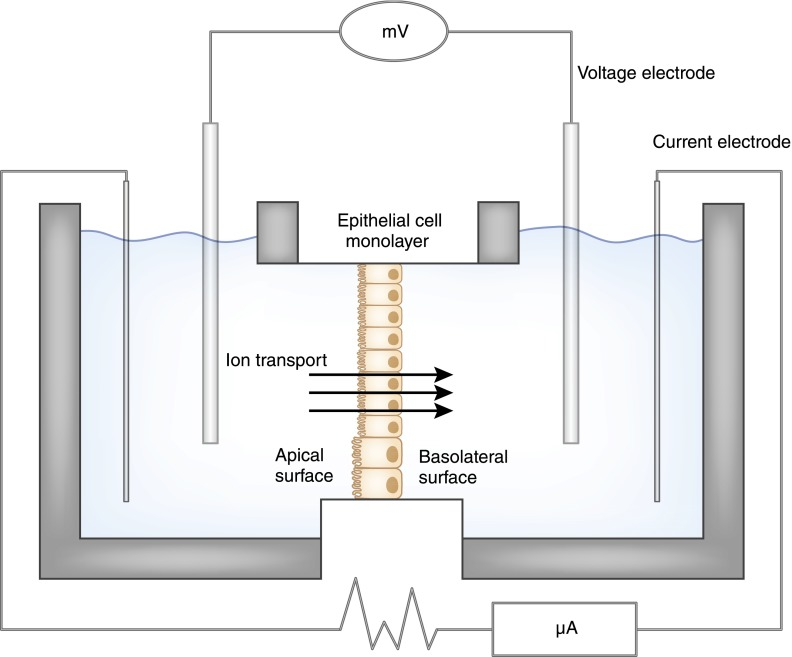
\includegraphics[width=1\textwidth]{figures/ussing_chamber.jpg}
	\end{center}
	\captionsetup{singlelinecheck = false, justification=raggedright}
	\caption[Ussing Chamber Setup] {\textbf{Ussing Chamber Setup}}{Ussing chambers can be used to characterise the function of a epithelial monolayer. The membrane can be exposed to different cellular conditions and its conductance can be measured under these conditions to test different drugs. Source \cite{hoenig2014}} 
\end{figure}

\subsubsection{Patch Clamp Electrophysiology}
\begin{figure}
	\label{patch_clamp}
	\begin{center}
	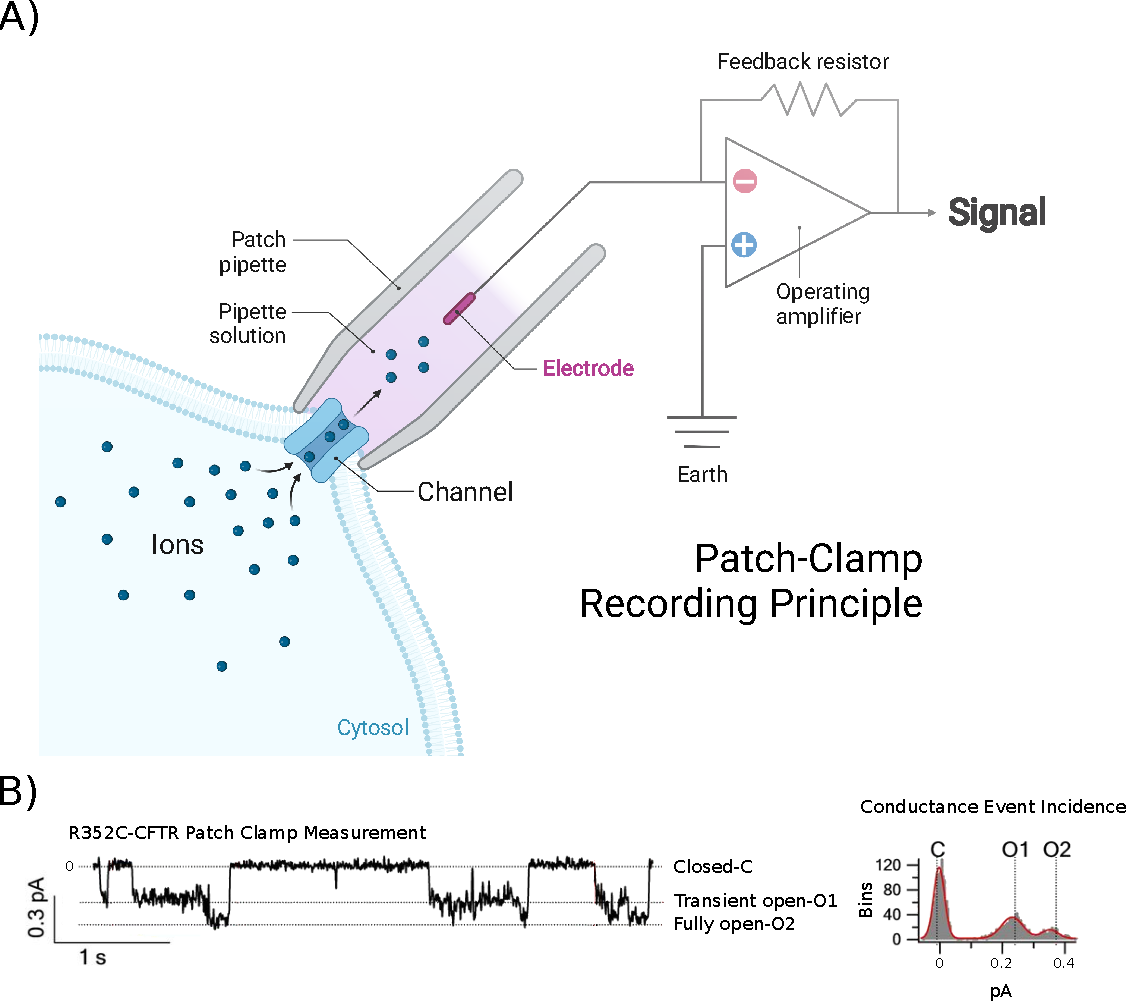
\includegraphics[width=0.6\textwidth]{figures/R352C_ephys_measurement_figure.pdf}
	\end{center}
	\captionsetup{singlelinecheck = false, justification=raggedright}
	\caption[Patch Clamp Apparatus] {\textbf{Patch Clamp Apparatus}}{A) In patch clamp electrophysiology, a micropipette is placed against the membrane to create a tight seal \cite{patch_clamp_recording_principal_figure}. B) The current trace from the measurement of a mutant CFTR channel. The R352C mutant was chosen for visualisation as it shows a clear transient state with lower conductance \cite{jih2012}. The accidental discovery of this mutant has been used extensively in studying the gating cycle of CFTR, giving an interesting example an example of how useful electrophysiology can be for molecular biophysics. Source data from \cite{jih2012}. Note that this mutant has roughly half the conductance of WT-CFTR.} 
\end{figure}
Patch Clamp Electrophysiology is a game changer for the molecular biophysics of ion channels. Through the use of a micropipette filled with electrolyte solution, we can measure the activity of a single ion channel. As shown in figure \ref{patch_clamp}, the pipette tip is placed directly on a cell membrane in order to measure the current flowing through a single ion channel. A single ion channel exhibits a current on the order of 1 picoAmp (for reference, CFTR exhibits 0.7pA at a bias voltage of 100 mV), so the formation of a tight seal with the membrane is critical to filter out noise. To tighten this seal, a small amount of suction is usually applied through the pipette \cite{aidley1996}.

In the inside-out variant of this technique, the ion channel along with a small patch of membrane is excised, exposing the system to the surrounding bath. This means that the response of the ion channel to different chemical conditions can be tested by changing the composition of the bath. PPatch clamp electrophysiology experiemnts are not presented in this thesis but they are heavily used in biophysical studies of CFTR so an explanation of their mechanism has been given here.

\subsection{Western Blotting Assesses CFTR Trafficking}
\begin{figure}
	\label{western_blot}
	\begin{center}
	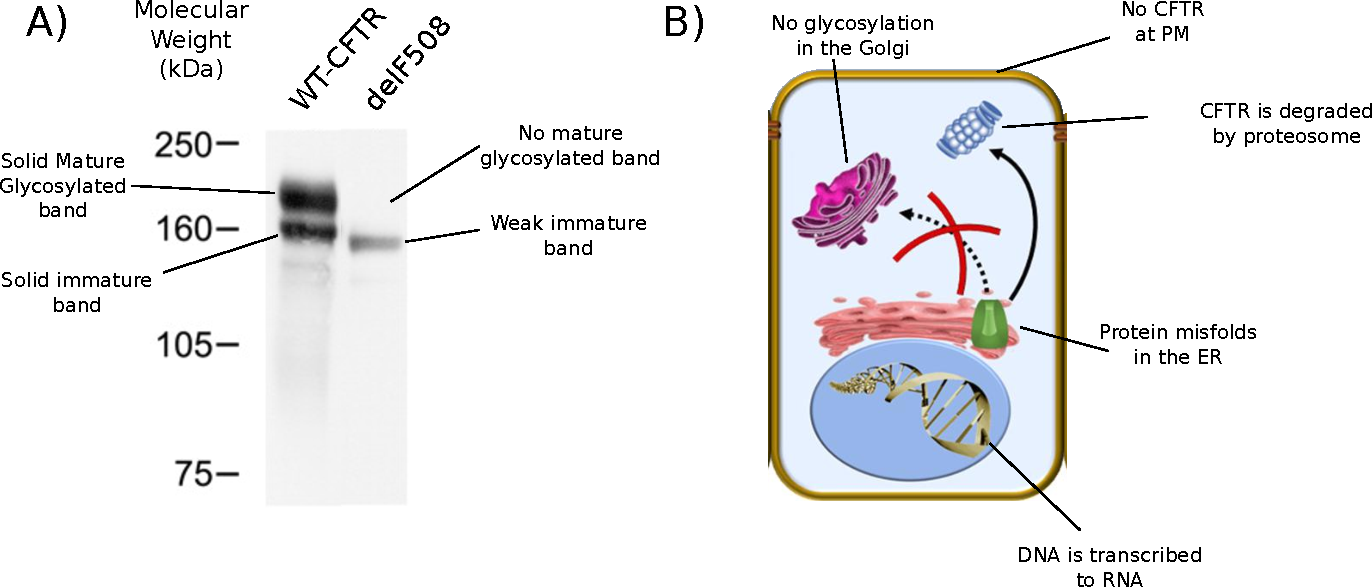
\includegraphics[width=1\textwidth]{figures/western_blot_explanation.pdf}
	\end{center}
	\captionsetup{singlelinecheck = false, justification=raggedright}
	\caption[Western Blot Explanation] {\textbf{Western Blot Explanation}}{A) Output of a western blot experiment. WT-CFTR has much more abundant protein than delF508 \cite{chang2008}. B) The cell biology behind why the delF508 mutation is pathogenic. When WT-CFTR folds correctly in the Endoplasmic reticulum it is trafficked into the Golgi where it is glycosylated, before it is then implanted into the cell membrane. In the case of delF508, the protein misfolds as it is synthesised, so instead of being trafficked as normal it is prematurely degraded by the proteosome \cite{lopes-pacheco2016a}.} 
\end{figure}
The above methods focus on measuring the electrical activity of the ion channels once they are at the cell membrane, they will only detect functional channels. In order to test the presence of ion channels within the epithelium, functional or otherwise we employ a technique called western blotting. See figure \ref{western_blot} to see how this can help us understand how measure the amount of protein at the cell surface. 

A simplified explanation is given below
\begin{enumerate}
	\item The proteins in the sample are denatured, sometimes by boiling, so they unfold and stretch out into long peptides. 
	\item The proteins in the sample are injected into a gel.
	\item The gel is immersed in a buffer solution and a voltage is applied to it in a process known as electrophoresis. This causes proteins to migrate through the gel according to their charge to mass ratio. The heavier the protein, the less it will move. 
	\item The presence of proteins is visualised through immunostaining. First, the gel is washed with a primary antibody. This antibody is specific protein we wish to detect (in our case, CFTR). 
	\item The excess primary antibody is washed off the gel, but some of the antibodies will stay bound to the proteins we are interested in. 
	\item A secondary antibody is washed over the gel. This is engineered to bind to the primary antibody. What is important about the secondary antibody is that it is attached to a special enzyme tag which we can visualise.  
	\item The excess secondary antibody is washed off the gel, but but some of the secondary antibodies will remain bound to the primary antibody.
	\item The tag on the secondary antibody is visualised through the use of chemiluminesence. The tag is typically an enzyme, which emits light when it breaks down a substrate. Hence, for the visualisation step, a photographic film is placed over the gel and it is washed one final time in the substrate of the enzyme which the secondary antibody is attached to. This produces bands in the photographic film, the darker the band is bound at that position, and the more protein is present.
\end{enumerate}
By washing the gel in different  primary antibodies, we can detect multiple proteins in one experiment. This is often used to normalise the amount protein quantity between samples, so you will often see structural proteins such as tubulin or actin in plots. These are used as controls and should not change due to most mutations. Western blotting is thus a simple, widely used technique to quantify the amount of specific proteins in the cell. 

\section{Conclusion}
As we have seen, CF is a complex disease. But its cause is relatively straight forward, disease arises from the misfunction of CFTR. This gives us some hope that by carefully understanding this protein system we can drastically improve the lives of many patients---while simultaneously developing an understanding of molecular biophysics. 

In subsequent chapters we will give careful examples of how to by closely integrating \textit{in silico} techniques with functional experiments in order to . With the detailed knowledge of CFTR that these studies give us, we will argue for a physics inspired model for the action of CFTR modulators in the broader context of the protein's molecular function. 

The combination of the above methods allows us to distinguish between the different classes of mutation which we outlined in section \ref{mutation_classes}. In the next 4 chapters we will make strong use of the these techniques to characterise, in detail, the nature of 4 rare CF causing mutations. This will help us better understand the action of small molecule drugs and how they can be used and developed to treat even more patients.

Note throughout the chapters ahead how we have made strong use of the careful biochemical and biophysical experiments which elucidate the molecular details of the function and misfunction of CFTR. The careful reading of these detailed studies was necessary in order to form hypothesise about the function of CFTR which we could test \textit {in silico}. As biophysics more closely integrates the keyboard with the benchside it will continue to be critical to consider \textit{in vitro} findings and so we are grateful to the painstaking work of Paul Linsdell, Christine E. Bear, Robert Ford, Laszslo Csandy, Tzyh-Chang Hwang, Naels Mccarty, Isabelle Callebaut, John Paul Mornon, David Gadsby, Jue Chen, Ina Urbatsch, John Hunt, Julie D. Foreman Kay and all the members of their laboratories for their careful studies of this fascinating protein. This is not to discount the work which went into the identification of the CFTR gene \cite{riordan1989}, nor the outstanding work of the clinicians and physicians who work with patients to understand more about the nature of the disease.  

Like we said in the Foreword \ref{chap:foreword}, we must all work together to understand the whole organism and thanks to the decades of work by hundreds of people we have a host of molecular details which we can combine in order to understand the function and misfunction of CFTR. In the next 4 chapters we will combine some of these details, alongside our own findings from organoid studies and simulations to make our own contribution to the molecular understanding of Cystic Fibrosis as a disease. This literature will again be used for our conclusion in chapter \ref{chap:conclusion} to push for certain questions to be answered in molecular CF research.
